%%%%%%%%%%%%%%%%%%%%%%%%%%%%%%%%%%%%%%%%%
% Journal Article
% LaTeX Template
% Version 1.4 (15/5/16)
%
% This template has been downloaded from:
% http://www.LaTeXTemplates.com
%
% Original author:
% Frits Wenneker (http://www.howtotex.com) with extensive modifications by
% Vel (vel@LaTeXTemplates.com)
%
% License:
% CC BY-NC-SA 3.0 (http://creativecommons.org/licenses/by-nc-sa/3.0/)
%
%%%%%%%%%%%%%%%%%%%%%%%%%%%%%%%%%%%%%%%%%

%----------------------------------------------------------------------------------------
%	PACKAGES AND OTHER DOCUMENT CONFIGURATIONS
%----------------------------------------------------------------------------------------

\documentclass[twoside,twocolumn,12pt]{article}

\usepackage{blindtext} % Package to generate dummy text throughout this template 

\usepackage[sc]{mathpazo} % Use the Palatino font
\usepackage[T1]{fontenc} % Use 8-bit encoding that has 256 glyphs
\linespread{1.5} % Line spacing - Palatino needs more space between lines
\usepackage{microtype} % Slightly tweak font spacing for aesthetics

\usepackage[english]{babel} % Language hyphenation and typographical rules

\usepackage[hmarginratio=1:1,top=25mm,columnsep=20pt,left=25mm]{geometry} % Document margins
\usepackage[hang, small,labelfont=bf,up,textfont=it,up]{caption} % Custom captions under/above floats in tables or figures
\usepackage{booktabs} % Horizontal rules in tables

\usepackage{lettrine} % The lettrine is the first enlarged letter at the beginning of the text

\usepackage{enumitem} % Customized lists
\setlist[itemize]{noitemsep} % Make itemize lists more compact

\usepackage{abstract} % Allows abstract customization
\renewcommand{\abstractnamefont}{\normalfont\bfseries} % Set the "Abstract" text to bold
\renewcommand{\abstracttextfont}{\normalfont\small\itshape} % Set the abstract itself to small italic text

\usepackage{titlesec} % Allows customization of titles
\renewcommand\thesection{\Roman{section}} % Roman numerals for the sections
\renewcommand\thesubsection{\roman{subsection}} % roman numerals for subsections
\titleformat{\section}[block]{\large\scshape\centering}{\thesection.}{1em}{} % Change the look of the section titles
\titleformat{\subsection}[block]{\large}{\thesubsection.}{1em}{} % Change the look of the section titles

\usepackage{fancyhdr} % Headers and footers
\pagestyle{fancy} % All pages have headers and footers
\fancyhead{} % Blank out the default header
\fancyfoot{} % Blank out the default footer
\fancyhead[C]{5584F $\bullet$ May 2020 $\bullet$ Harvey Hughes} % Custom header text
\fancyfoot[RO,LE]{\thepage} % Custom footer text

\usepackage{titling} % Customizing the title section

\usepackage{hyperref} % For hyperlinks in the PDF

\usepackage{graphicx}
\graphicspath{ {images/} }

\newenvironment{reusefigure}[2][htbp]
  {\addtocounter{figure}{-1}%
   \renewcommand{\theHfigure}{dupe-fig}% If you're using hyperref
   \renewcommand{\thefigure}{\ref{#2}}% Figure counter is \ref
   \renewcommand{\addcontentsline}[3]{}% Avoid placing figure in LoF
   \begin{figure}[#1]}
  {\end{figure}}
\usepackage{wrapfig}
\usepackage{amsmath}
\usepackage{xcolor}
\usepackage{listings}
\usepackage{subcaption}
\usepackage{pdfpages}
\usepackage{array,multirow,graphicx}
\lstset{
  basicstyle=\ttfamily,
  columns=fullflexible,
  frame=single,
  breaklines=true,
  postbreak=\mbox{\textcolor{red}{$\hookrightarrow$}\space},
}

\newcommand{\threepartdef}[6]
{
	\left\{
		\begin{array}{lll}
			#1 & \mbox{: } #2 \\
			#3 & \mbox{: } #4 \\
			#5 & \mbox{: } #6 \\
			0 & \mbox{: } otherwise
		\end{array}
	\right.
}
\usepackage{multicol}
\usepackage{stfloats}

%----------------------------------------------------------------------------------------
%	TITLE SECTION
%----------------------------------------------------------------------------------------

\setlength{\droptitle}{-4\baselineskip} % Move the title up

\pretitle{\begin{center}\Huge\bfseries} % Article title formatting
\posttitle{\end{center}} % Article title closing formatting
\title{Robotic Unicycle} % Article title
\author{%
%\textsc{Final Report} \\
%\\
\textsc{Harvey Hughes} \\
\textsc{Supervisor:Professor Carl Rasmussen} \\
}
\date{\today} % Leave empty to omit a date
\renewcommand{\maketitlehookd}{%

}

%----------------------------------------------------------------------------------------

\begin{document}

% Print the title
\maketitle

%----------------------------------------------------------------------------------------
%	ARTICLE CONTENTS

\section*{Technical Abstract}
The application of machine learning to calculate a control policy opposed to using control theory could prove to be highly useful when its not possible to determine system dynamics. However, success outside of simulations has been slow. A robotic unicycle is considered in this project with tests into roll limit, sampling time, phone connection and initial orientation being tested first in order to brooch the gap between simulation and real success.

\clearpage
a
\onecolumn

%----------------------------------------------------------------------------------------
\tableofcontents

\twocolumn

\begin{figure*}[b!]
  \centering
  \begin{subfigure}[t]{0.325\textwidth}
    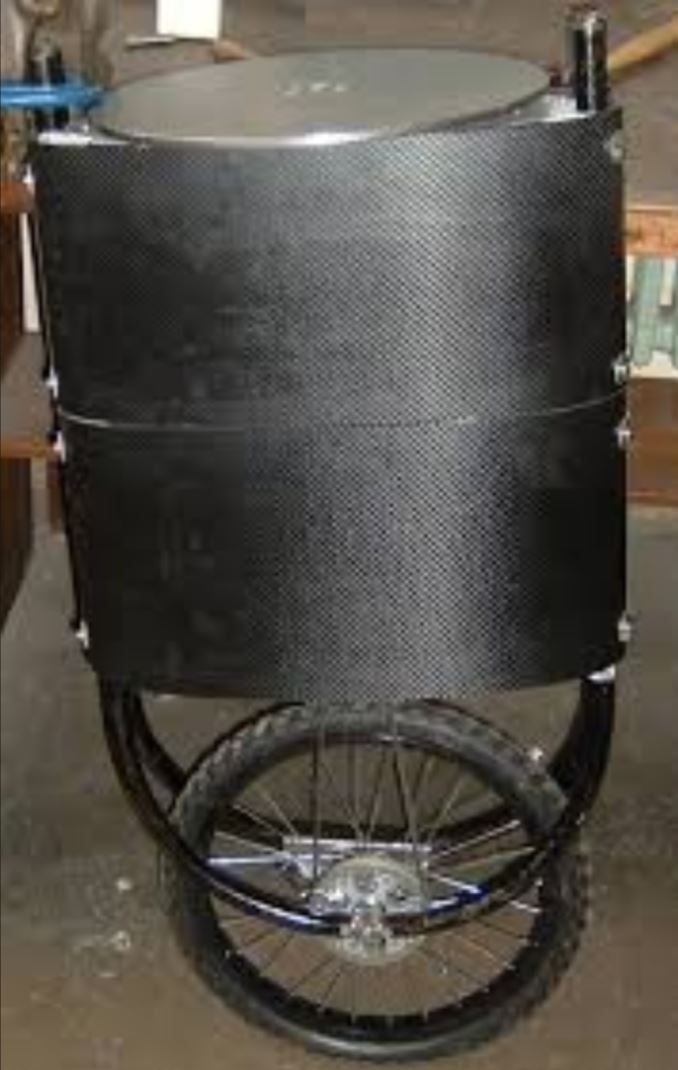
\includegraphics[width=\linewidth,height=7.5cm]{first}
   \caption{1m tall 1st model \cite{roderigo}}
  \label{sub:old1}
  \end{subfigure}
  \begin{subfigure}[t]{0.325\textwidth}
    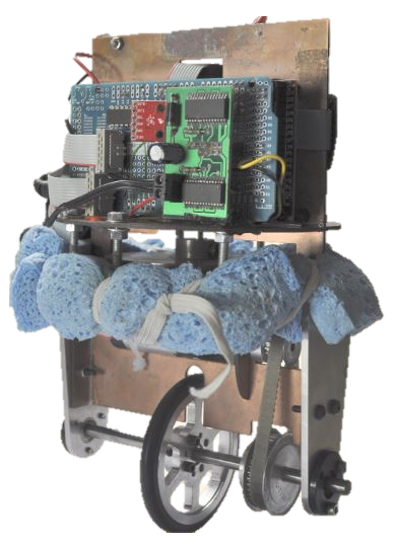
\includegraphics[width=\linewidth,height=7.5cm]{old_unicycle}
    \caption{20cm tall 2nd model \cite{eric}}
  \label{sub:old2}
  \end{subfigure}
  \caption{Previous unicycle iterations}
  \label{fig:unimodels}
\end{figure*}
\section{Introduction}
\subsection{Project aims}
\lettrine[nindent=0em,lines=3]{T}he aim of this project is to create a controller that is able to balance a robotic unicycle. The controller starts off with no information about the system, and is therefore required to slowly learn what are good actions to make. This mimics the way in which humans learn new tasks as children by trying new actions and seeing if they're beneficial.
\newline
This is an ongoing project from previous years where success has been shown in simulations yet has so far been hard to achieve in real life. A major outcome of this project is the build upon previous years work and fix existing issues, in addition to solving new ones in order to bring the success of a real unicycle closer to simulations. 
\newline
This project aims to demonstrate the effectiveness of implementing the PILCO algorithm \cite{pilco} on more complex dynamic systems. PILCO has previously been shown to tackle simpler problems such as a cart-pole system with less data and high speeds compared to other algorithms. 
\newline 
A unicycle is a suitable example to test on due to the complex nature of the problem, even for human riders. Balancing on the spot is additionally a less linear and therefore harder problem to solve then simply moving forward. This complexity allows the full extremes of the PILCO algorithm to be explored and therefore demonstrate all flaws and benefits in PILCO.
%---------------------------





\subsection{Previous work}
Work has been conducted on robotic unicycles within the engineering Department on and off since 2005 \cite{original}. This unicycle was full sized at 1m, and weighed 35kg shown in figure \ref{sub:old1}. Built by Mellors and Lamb the unicycle involved a wheel motor and horizontal flywheel motor to mimic the rotation arms can create. Having the flywheel in the horizontal plane increases the complexity over other designs with in in the vertical plane, as it couples the two motors together when a roll angle is corrected.
\newline
The problem was originally being solved using control theory approaches. This involved complex analysis of the dynamics in 2D and 3D conducted in 2007-2009 by D'Souza-Mathew \cite{neil} and Forster  \cite{forster}. Some success was demonstrated at balancing the unicycle. However, simplifications in the analysis resulted in non-linearities present in real life to not be considered accurately.
\newline
In 2010 Mchutchon \cite{mchut} applied the RMLC (Reinforced Model Learnt Control) algorithm developed by Rasmussen and Deisenroth to the unicycle, and acived balancing of a unicycle with stabilisers. In 2011 building upon Mchutcons work Queiro \cite{roderigo} and Douglass \cite{douglass} were able to modify the unicycle to balance unrestrained for up to 5 seconds. 
\newline
The size of the unicycle posed serious safety risks, both in terms of replacing large components and the need to limit the unicycle during tests. One way this was done was by attaching to bike racks \cite{neil} or suspending the unicycle from the department atrium \cite{roderigo}. These methods while reducing the risk didn't eliminate it, and caused unnecessary simplifications or disturbances to the unicycle dynamics. 
\newline
To increase safety a small model unicycle was constructed as in figure \ref{sub:old2}. PILCO was also implemented on the unicycle \cite{pilco}. The increased safety of the smaller unicycle allowed unconstrained motion to be tested more easily. Work began on the miniature unicycle in 2015 by Tukiainen \cite{tuk}. Problems in balancing the unicycle were encountered at this point, with concerns about identifying the cause for problems. In 2017 an overhaul of the software was done by Wieser \cite{eric}, and in 2019 an electrical overhaul by Harris \cite{arsalan}. This was to simplify the system and allow for more accurate troubleshooting. 

\begin{figure*}[t!]
  \centering
  \begin{subfigure}[t]{0.325\textwidth}
    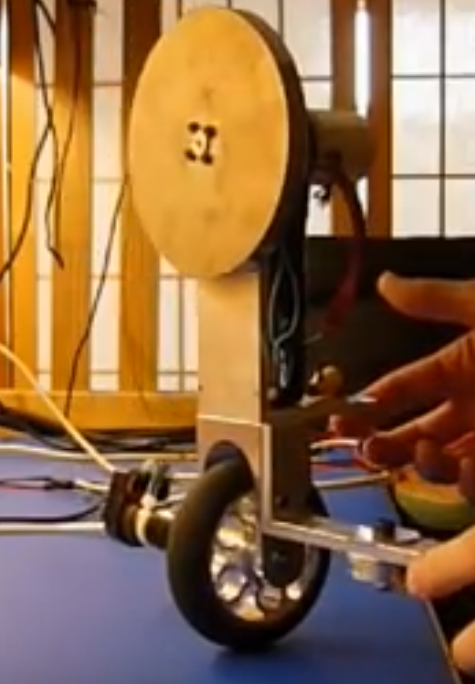
\includegraphics[width=\linewidth,height=7.5cm]{other1}
   \caption{\cite{other1}}
  \label{sub:oother1}
  \end{subfigure}
  \begin{subfigure}[t]{0.325\textwidth}
    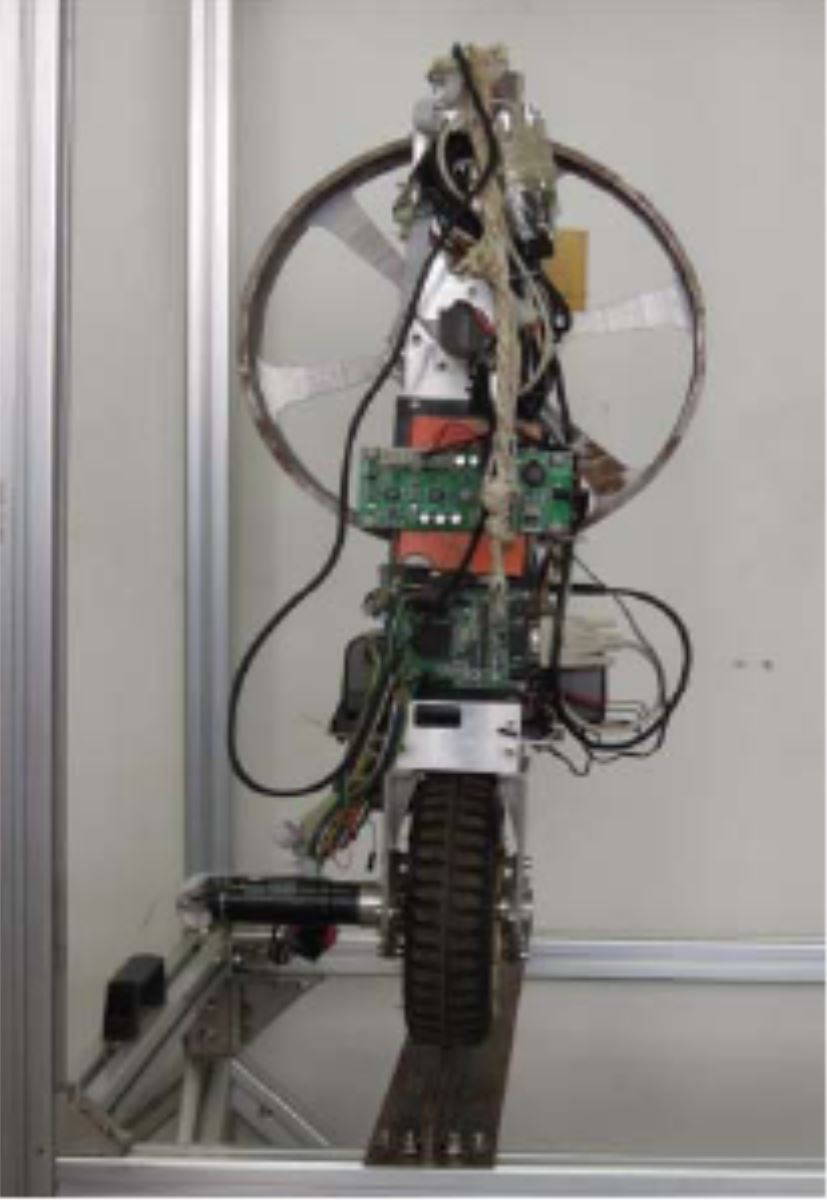
\includegraphics[width=\linewidth,height=7.5cm]{other3}
    \caption{\cite{other2}}
  \label{sub:other2}
  \end{subfigure}
  \caption{Other Unicycle designs}
  \label{fig:otheruni}
\end{figure*}

%---------------------------
\subsection{Examples of other unicycles}
There are numerous examples of other work conducted on balancing robotic unicycles. Many of these involved a large vertical flywheel and use of control theory as seen in figure \ref{fig:otheruni}. Orientating the disk this way improves stability and was therefore quite successful at balancing. The improved stability is due to uncoupling the two torques, meaning that to correct a roll error just the flywheel can be used, and to correct a pitch error the wheel only needs rotating. A combination of both actions is required to fix roll errors on a unicycle with horizontal flywheel.



There has been work done on unicycles set-up with a horizontal flywheel. \cite{other3}. Vos and Von Flotow analysed a large unicycle and were able to balance to some success. This required multi region control policies to work, and therefore was very complicated.
\newline
The robotic unicycles discussed so far have all been developed using traditional control theory. Very few unicycles have been controlled with a machine learning approach. Simulations of a 2D unicycles were successfully balanced \cite{other4} using standard keras and Tensorflow libraries. However, this approach simplifies the problem back to a much easier inverted pendulum, and didn't deal with the problems associated with real models. The lack of previous success at this particular task highlights its difficulty.

%------------------------------------------------
\clearpage
\section{Theory}
\subsection{Coordinate System}
In order to fully define the unicycle state at each time step seven coordinates and their derivatives are required. These coordinates are shown in figure \ref{fig:ang} giving the state as

\begin{align*}
\textbf{x} = [\dot{x} \: \dot{y}\: \dot{\theta}\: \dot{\phi}\: \dot{\psi}_f\: \dot{\psi}_w \:\dot{\psi}_t \: x \: y \: \theta \: \phi \: \psi_f \: \psi_w \: \psi_t]^T
\end{align*}


\begin{figure}[h]
  \centering
  \begin{subfigure}[t]{0.1935\textwidth}
    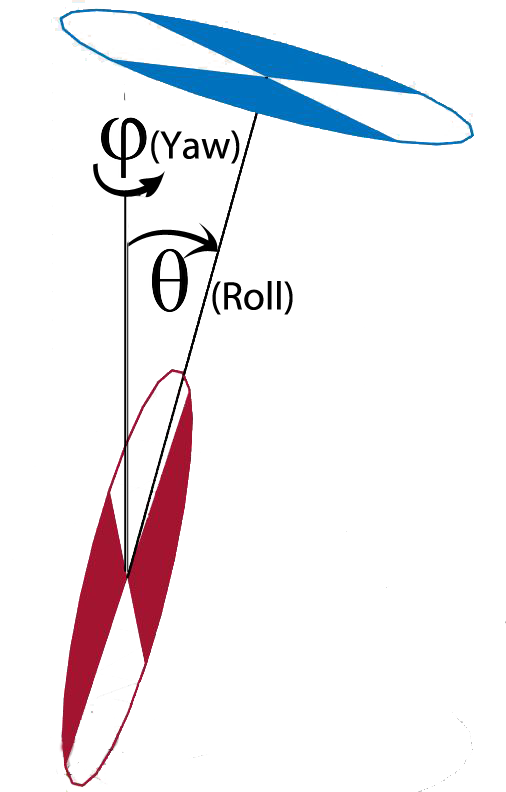
\includegraphics[width=\linewidth]{end_labled2}
  \label{fig:e}
  \end{subfigure}
  \begin{subfigure}[t]{0.2295\textwidth}
    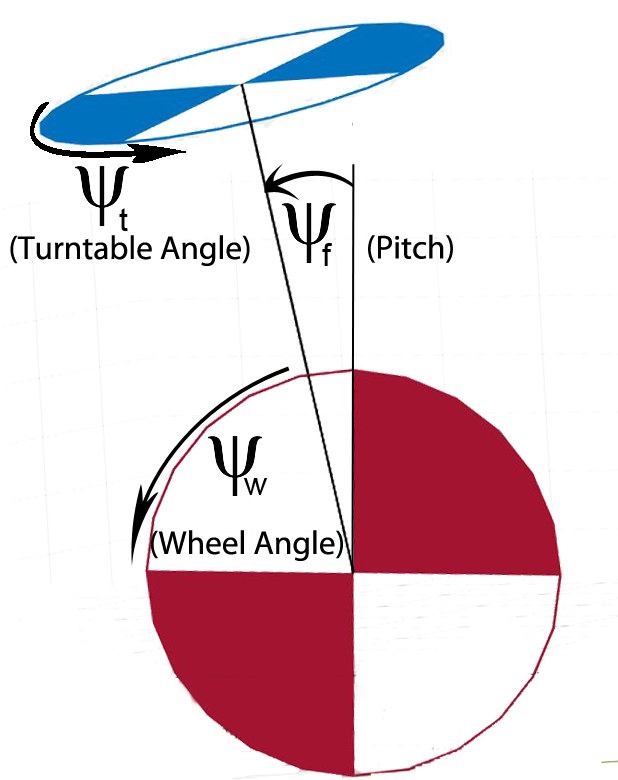
\includegraphics[width=\linewidth]{side_labled}
  \label{fig:s}
  \end{subfigure}
  \caption{Angles used to define position}
  \label{fig:ang}
\end{figure}

In order to define rotations in 3D to represent $\theta,\phi,\psi_f$ correctly care must be taken to the order the rotations are applied. This is because rotations are non commutative in 3D unlike in 2D. The convention of Euler angles is used to solve this problem. \cite{eric}
\newline
There are 12 orders of rotation which can be used. XYZ or 123 convention is used on the unicycle as in equation \ref{eq:eul}. Where $R_A(\alpha)$ represents a right hand rotation about axis A of $\alpha$. 

\begin{equation}
R_{XYZ}(\psi_f,\theta,\phi)\textbf{x} = R_X(\psi_f)R_Y(\theta)R_Z(\phi)\textbf{x}
\label{eq:eul}
\end{equation}

%-------------------------------
\subsection{Quaternions}
As discussed previously rotations in 3D are difficult to combine due to their non-commutative nature. A handy way of dealing with consecutive rotations is to use quaternions. These are an extension of complex numbers to include three imaginary parts and are written as:

\begin{align*}
a + b\textbf{i} + c\textbf{j} + d\textbf{k}
\end{align*}

The following properties allow quaternions obey the same rules as 3D rotations:

\begin{align*}
\textbf{i}^2 = \textbf{j}^2 = \textbf{k}^2 = \textbf{ijk} = -1
\end{align*}

A rotation about axis (x,y,z) by $\alpha$ can be defined using the following unit quaternion \cite{quat}

\begin{gather}
\textbf{q}_{rot} = cos(\frac{\alpha}{2}) + sin(\frac{\alpha}{2})x\textbf{i} + sin(\frac{\alpha}{2})y\textbf{j} + sin(\frac{\alpha}{2})z\textbf{j} \nonumber \\
\textbf{q}_{new} = \textbf{q}_{old} . \textbf{q}_{rot} \nonumber
\end{gather}

%----------------------------------
\subsection{Optimal Control}
 
 
%--------------------------------------------------------

\subsection{PILCO}
In policy optimisation an algorithm called PILCO \cite{pilco} will be used.
This method will optimise a policy to decide the best action $\textbf{u}$ given the unicycles state. To determine optimum actions the expected loss over a horizon is evaluated under the current policy, as in equation \ref{eq:pilco}.


\begin{equation}
\begin{split}
\pi^*(\textbf{x}) = argmin \sum_0^tc(\textbf{x}^{(i)}) \\
\textbf{u}^{(i)} = \pi(\textbf{x}^{(i)} )\\
\end{split}
\label{eq:pilco}
\end{equation}


%-----------------------------------
\subsection{Gaussian Processes}

A Gaussian process is used to model the dynamics and gives a range of possible functions which fit observed data in a non parametric way as to not introduce model bias. A Gaussian process is a generalisation of a multivariate Gaussian to infinitely many variables. As a result a mean and covariance function are used to define it as in equation \ref{eq:gp}.
\begin{equation}\label{eq:gp}
\begin{gathered}
f(\textbf{x}) \sim \mathcal{GP}(m(\textbf{x},k(\textbf{x},\textbf{x'})) \\
m(\textbf{x}) = \mathbb{E}[f(\textbf{x})]  \\
k(\textbf{x},\textbf{x'}) = \mathbb{E}[(f(\textbf{x})-m(\textbf{x}))( f(\textbf{x'})-m(\textbf{x'}))]
\end{gathered}
\end{equation}

A major advantage of PILCO is the ability to retain uncertainty throughout this process. This means an initial state distribution can be propagated forward to generate a state distribution at each time step. These distributions are used to calculate the average instantaneous cost in policy evaluation.
The uncertainty grows over time and comes from an initial variation in start position, measurement noise, and process noise. 

\begin{figure}[h]
  \centering
  \begin{subfigure}[t]{0.5\textwidth}
    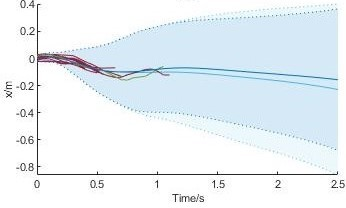
\includegraphics[width=\linewidth]{u2}
  \caption{x Prediction} 
  \label{sub:ffffffs}
  \end{subfigure}
  \begin{subfigure}[t]{0.5\textwidth}
    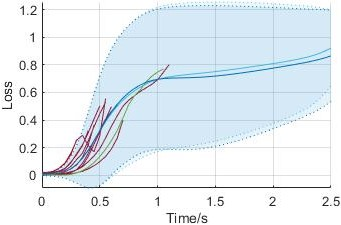
\includegraphics[width=\linewidth]{loss2}
  \caption{Loss prediction}
  \label{sub:ffs}
  \end{subfigure}
  \caption{Predictions from PILCO approach}
  \label{fig:pilco}
\end{figure}

Figure \ref{sub:ffffffs} shows predicted x position, with predictions up to 0.5s showing low uncertainty. After this the model loses the ability to predict the state accurately and the state distribution widens. 
A similar trend is observed for the predicted loss at each time step in figure \ref{sub:ffs}.
\newline
PILCO uses an iterative approach to optimising policy. Initially a random controller is used to get sufficient data for a dynamic model. Policy optimisation and rollouts under the new policies can then occur until the task is either learnt or terminated. 


%---------------------------------------------------------------
\subsection{Cost Function}
A cost function is required to evaluate the performance at each timestep. This takes the form of equation \ref{eq:simple}. Where a, h and $\theta_{max}$ represent positive constants, and d(\textbf{x}) is the geometric distance of the unicycle tip from the starting position.


\begin{equation}
\label{eq:simple}
\begin{gathered}
c(\textbf{x}) = 1 - \mathcal{R}(\textbf{x}) \\ 
\mathcal{R}(\textbf{x}) = exp(-\frac{a}{2h^2}d(\textbf{x})^2 - \frac{\phi^2}{2(4\pi)^2} - \frac{\theta^2}{\theta_{max}^2}) 
\end{gathered} 
\end{equation}
%------------------------------------------

\clearpage

\begin{figure*}[t!]
  \centering
  \begin{subfigure}[t]{0.325\textwidth}
    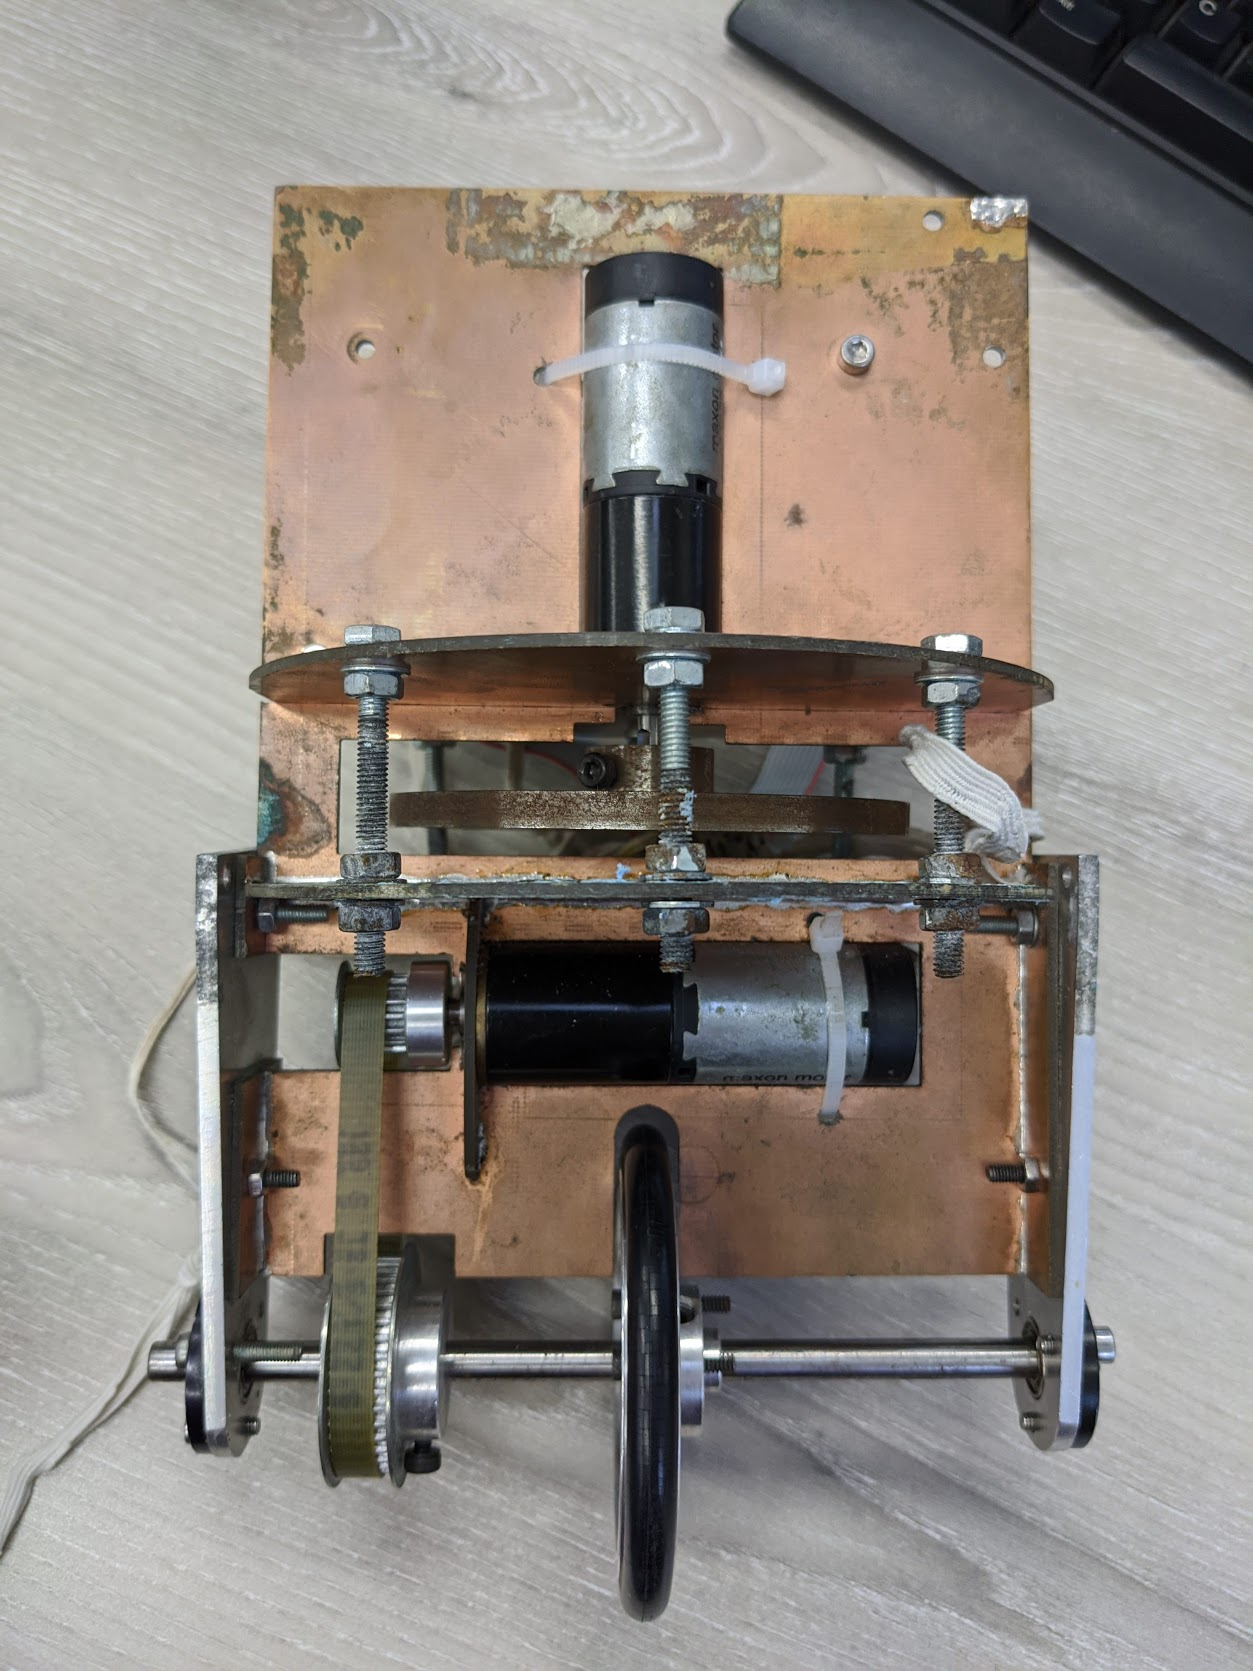
\includegraphics[width=\linewidth,height=7.5cm]{uni_old_mech}
   \caption{Frame}
  \label{sub:frameold}
  \end{subfigure}
  \begin{subfigure}[t]{0.325\textwidth}
    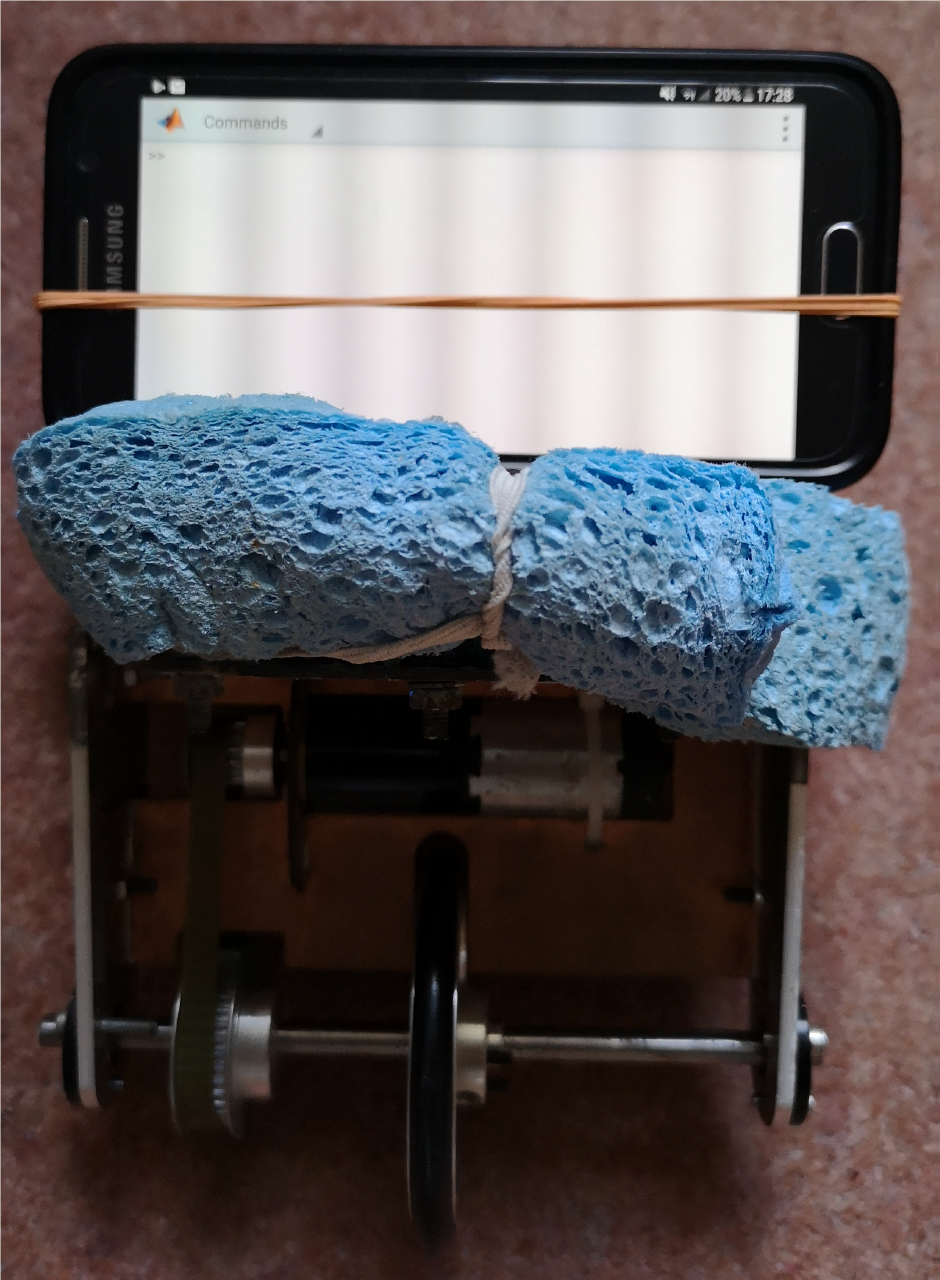
\includegraphics[width=\linewidth,height=7.5cm]{old1}
    \caption{Front \cite{arsalan}}
  \label{sub:frontold}
  \end{subfigure}
  \begin{subfigure}[t]{0.325\textwidth}
    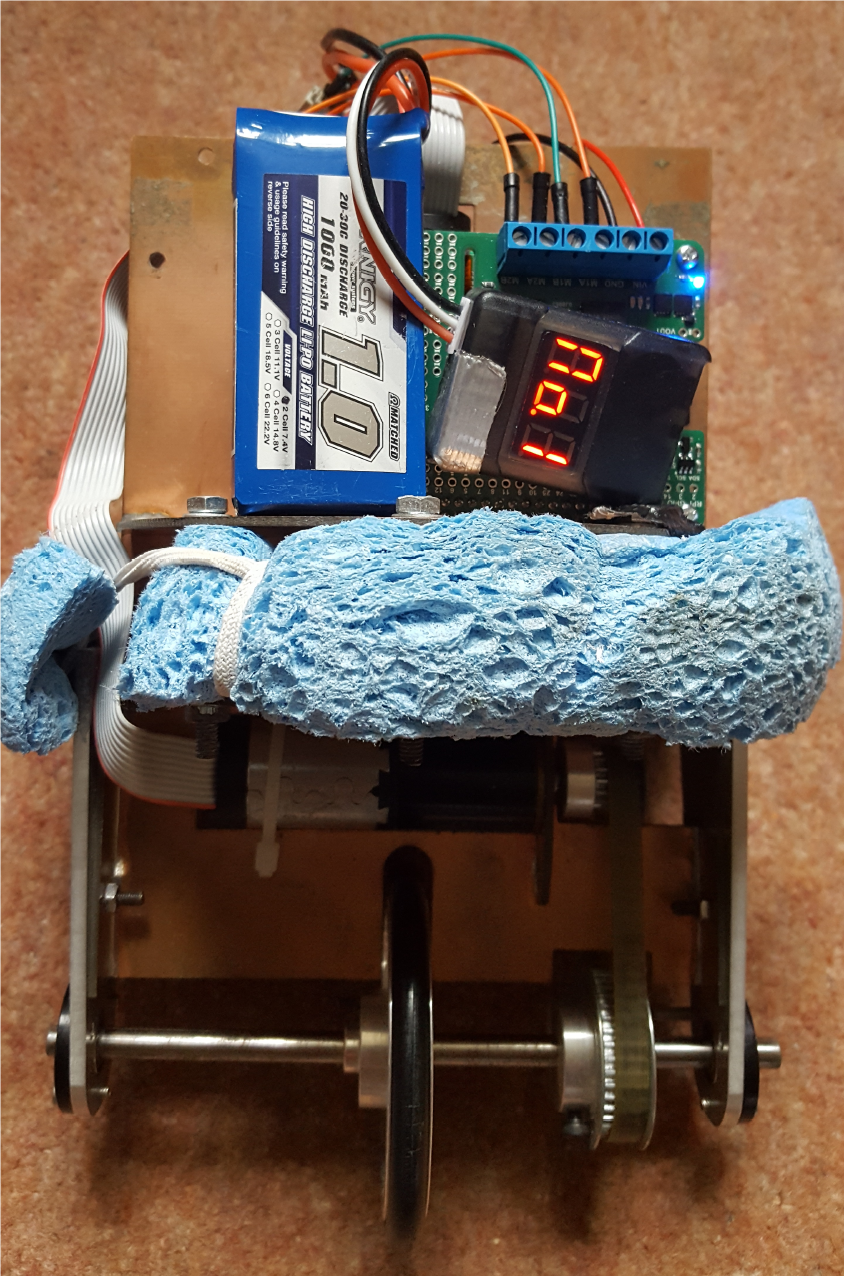
\includegraphics[width=\linewidth,height=7.5cm]{old2}
    \caption{Back \cite{arsalan}}
  \label{sub:backold}
  \end{subfigure}
  \caption{Current set-up of unicycle}
  \label{fig:current}
\end{figure*}
need to label the images and probs make them bigger?

\section{Current Unicycle Set-up Review}
\subsection{Mechanical}
Figure \ref{sub:frameold} shows the mechanical design of the unicycle. The unicycle was built from PCB boards made of copper coated fibreglass and subsequently welded together. This material was very light and stiff and helped keep the overall weight to about 1.2kg. The unicycle stands at 20cm tall in real life.
\newline
Two identical motors are used on the unicycle, these are Maxon ..... \cite{maxonmotor}. These motors have maximum continuous torques of 6.31mNm and speeds of ....rpm. These motors run fast so to improve sensitivity and increase torque output a 14:1 planetary gearhead \cite{gearhead} is attached to each motor. To further increase torque output on the wheel a gearing of 40:16 is implemented via a belt. This results in maximum output torques of the motors as 0.205Nm and 0.513Nm for the turntable and wheel respectively. Each motor has an attached encoder which pulses 512 times per revolution, this can be used to accurately track the motor positions but is currently not in use.
\newline
The flywheel of the unicycle is mounted horizontally and cased within the frame to prevent injury and damage to the motors.
\newline
To prevent damage to the unicycle when falling a basic protection of foam was added to the unicycle. The unicycle currently crashed when a roll angle of $17^{\circ}$ or pitch of $75^{\circ}$ is achieved. 
\subsection{Electrical}
The electrical components on the unicycle was simplified by Harris \cite{arsalan} to only involve a phone, Raspberry Pi and Raspberry Pi motor board. This simplification was to reduce the number of components required to be brought together for successful rollouts, helping reduce complexity and increase ease of troubleshooting. 
\newline
The phone is used to take advantage of high quality sensors existing in a device most people own. The on-board gyroscope is used to measure the current state, with the possibility of using the other sensors such as accelerometer to calculate initial position. 
\newline
The Rasberry Pi is used to control the motor torques via the attached motor board. This replaced a normal micro controller and was chosen to allow future adaptability in design as a Raspberry Pi has lots of additional functionality over a micro controller.
\newline
The phone and Pi were unreliability attached using rubber bands. This introduced lots of additional noise as the sensor could move between rollouts or during a rollout, therefore effecting the generalisation of learnt dynamics to all rollouts. To minimise this problem the phone was realigned by attaching and reattaching before each trial. 
\begin{figure*}[t!]
  \centering
    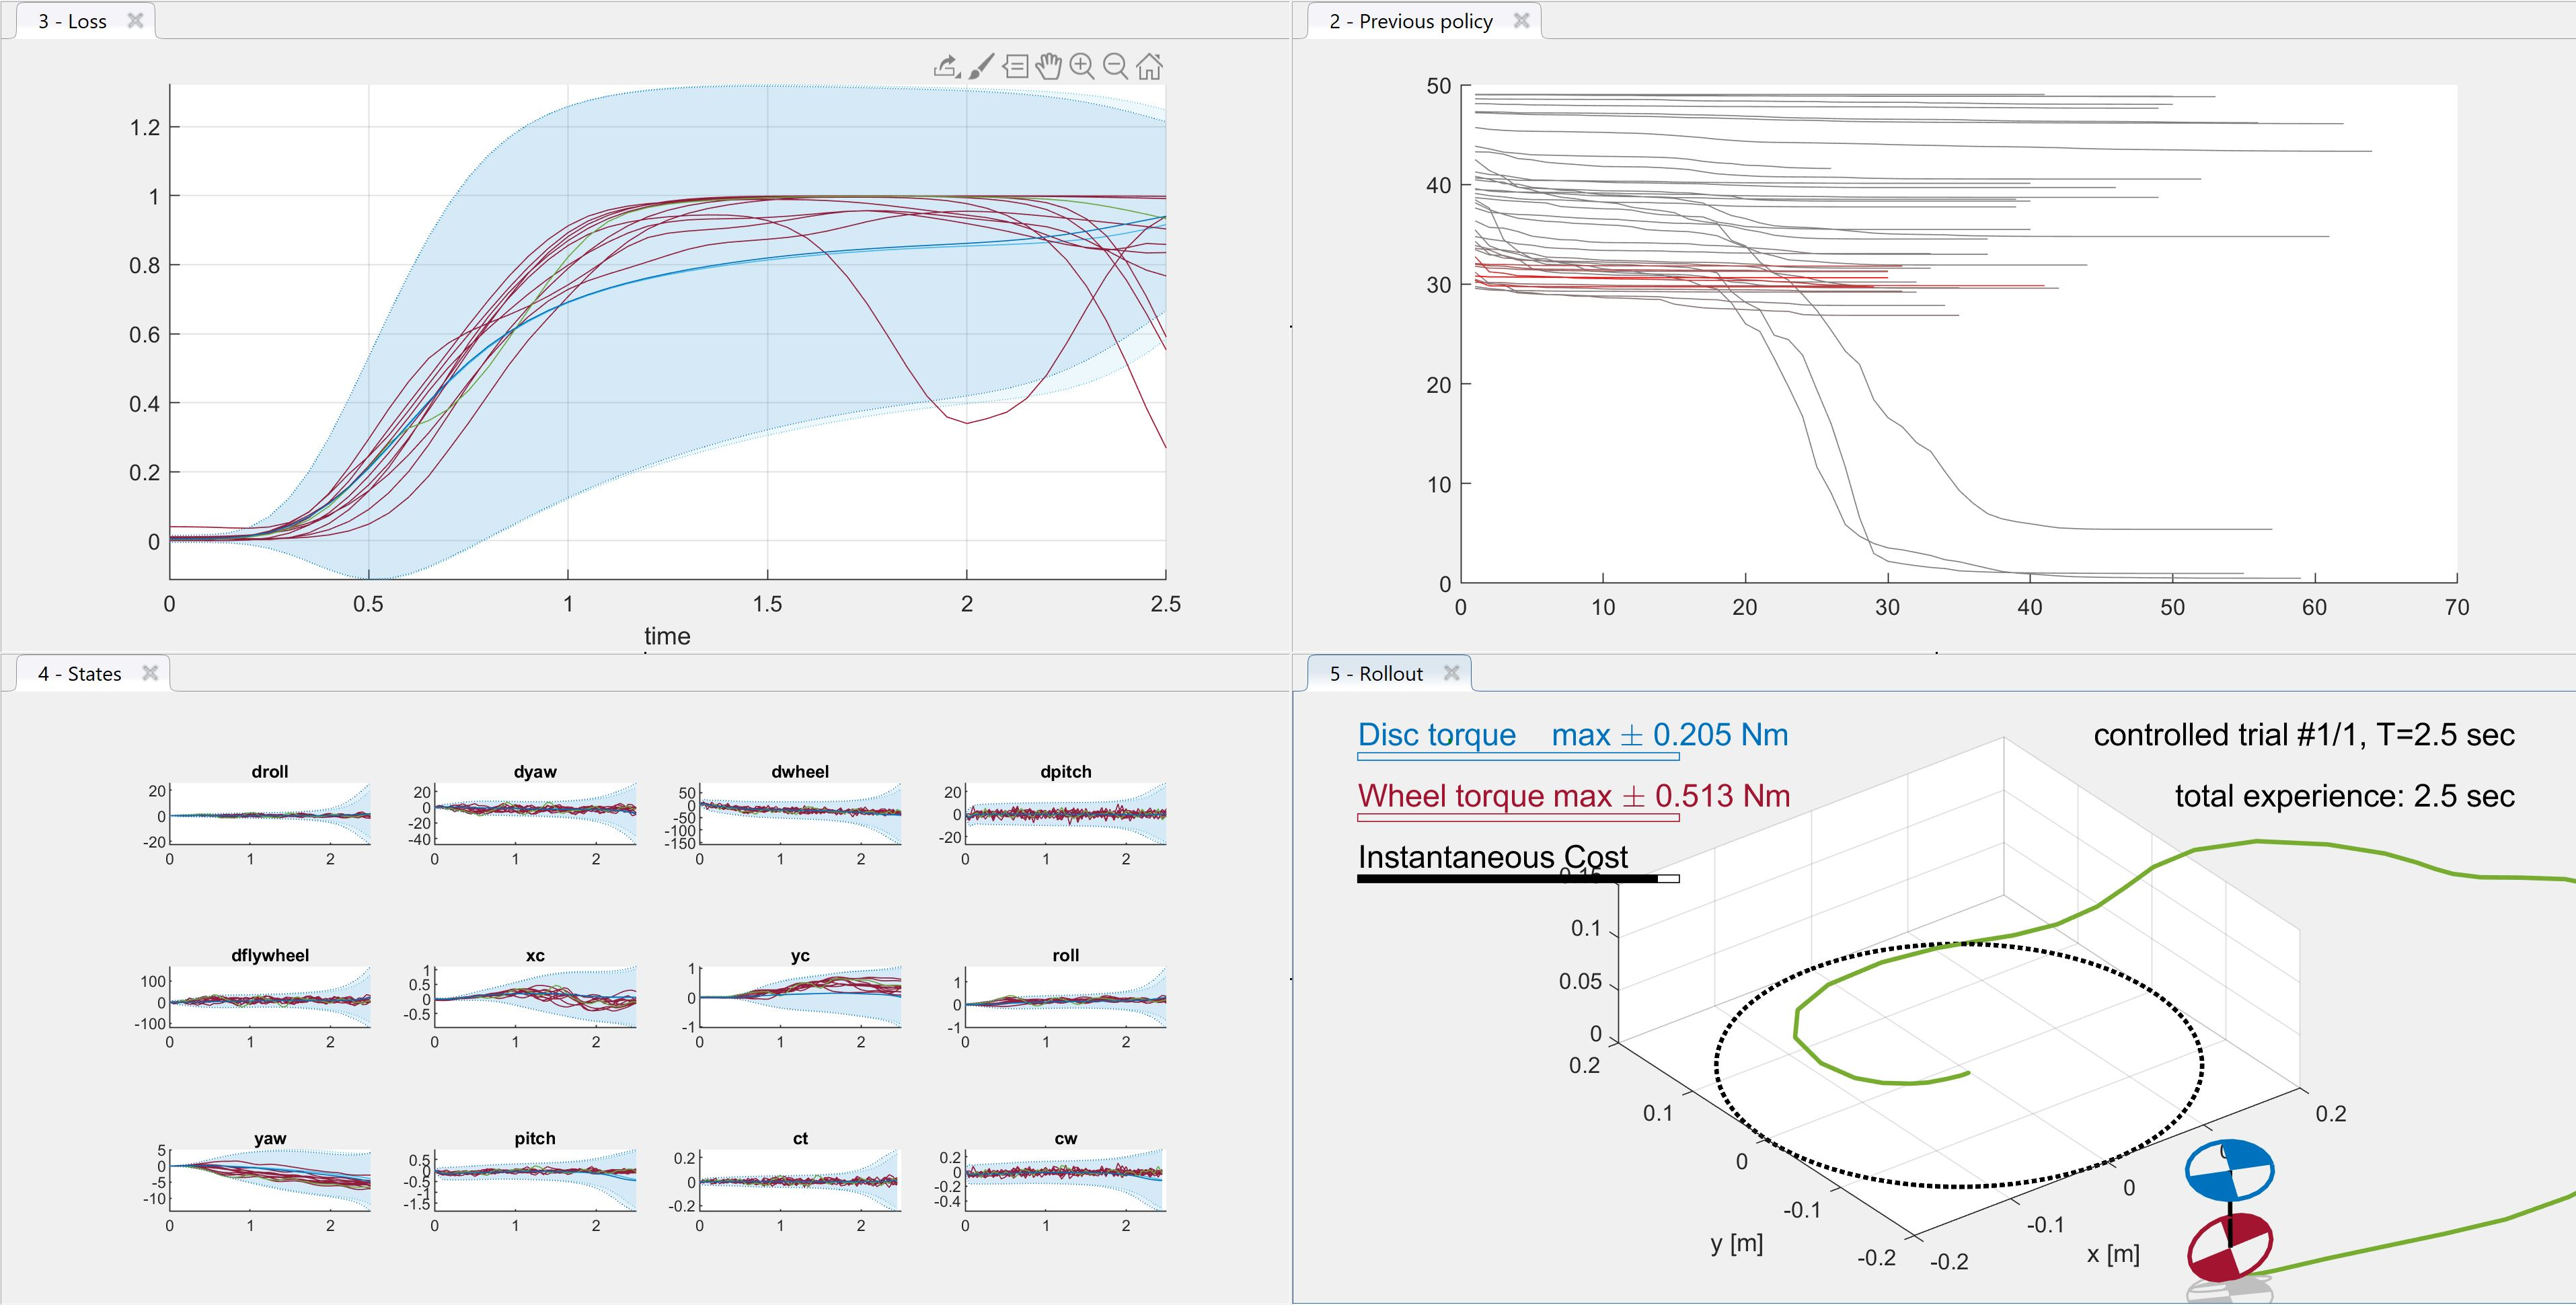
\includegraphics[width=\linewidth]{pilco}
   \caption{Information displayed during rollouts}
  \label{fig:pilcoscreen}
\end{figure*}
\subsection{Software}
The main body of the code is run in Matlab on an attached computer. This code is part of the extensive PILCO toolbox, the following steps are required when programming a scenario in PILCO, with each step using the structures and methods defined in the package.

\begin{itemize}
\item Define all state variables, including policy and dynamics inputs and outputs, variables solved for when simulating and which variables correspond to angles
\item Number of rollouts to optimise policy over 
\item Number of random rollouts
\item horizon time
\item Initial state distribution, including state uncertainties
\item Policy structure, and optimisation methods
\item Plant information including simulation dynamics
\item Controller structure
\item Dynamics function structure and optimisation
\item Cost function
\item Optional policy exploration methods
\item Iterations of learning dynamics from new rollouts, then optimising policy function for use in next rollout can then occur.
\end{itemize}



Figure \ref{fig:pilcoscreen} shows the information generated during rollouts. Shown in these plots is the states, loss, unicycle animation, and policy improvements across rollouts. The state window shows the trajectory of 10 rollouts under the current policy, with the rollout used in training displayed in green. The predictive state uncertainty and mean is displayed in light blue, with the dark blue indicating an updated prediction after re optimising the dynamics function using the new data. Multiple rollouts are displayed to get a better idea about the behaviours exhibited by the controller, and to check the chosen rollout is typical. The loss window shows the same 10 rollouts and the cost distribution expected at each timestep. The animation displays the unicycle trajectory and traced path for the green rollout, the current actions and cost is also displayed. Policy learning can be analysed by looking at the policy window. This displays the expected loss, optimized 100 times, for each policy iteration. A horizontal line, or grouping of consecutive policy lines can indicate a reduction in learning rate. Often when little data has been observed the trajectory predictions can be overly optimistic, causing the predicted loss decrease rapidly in some iterations. This prediction is later reverted once more data has been observed.   Additional features such as replaying an animation can be performed by right clicking the desired trajectory line in the GUI, described in detail in by Weiser \cite{eric}. 
Log files are generated of each rollout to allow for easy post processing or reusing old data on modified algorithms.
\newline
During rollouts sensor readings from the phone were logged and used within Matlab by using a now discontinued feature of Matlab mobile. This feature allowed the connection of a phone and computer logged into the same Matlab account to share data eg sensor readings over wifi.
\newline
Position calculations and subsequent policy evaluations were then performed within Matlab to determine the motor input torques. These were called using the following commands \cite{arsalan}: 
\begin{itemize}
\item system(mypi, 'sudo python m/enabling\_motors.py')
\item system(mypi, 'sudo python m/motor\_contorl\_2.py -240 120')
\item system(mypi, 'sudo python m/disabling\_motors.py')
\end{itemize}
These commands opened a command terminal on the Pi through Matlabs integration to Pi package. In this terminal python files could then be executed to turn motors on/off, or change speeds.
%----------------------------------

\clearpage
\section{Initial Simulation Results}

During previous years the Unicycles performance on the real model was relatively poor. A mechanical redesign was considered to fix some of these issues. In order to evaluate the performance of this redesign and additional factors simulations were conducted as they allowed a quick and easy way to alter variables.
\newline

%-------------------------------
\subsection{Test Procedure}

Two different measures will be used to determine success. The first being time upright as more rollouts occur. This is to determine any success at balancing the model has. The second is total rollout loss in order to see if success is achieved by staying near the origin instead of staying upright.
%......................................................
\subsection{Roll Limit}
\begin{figure*}[ht!]
  \centering
  \begin{subfigure}[t]{0.325\textwidth}
    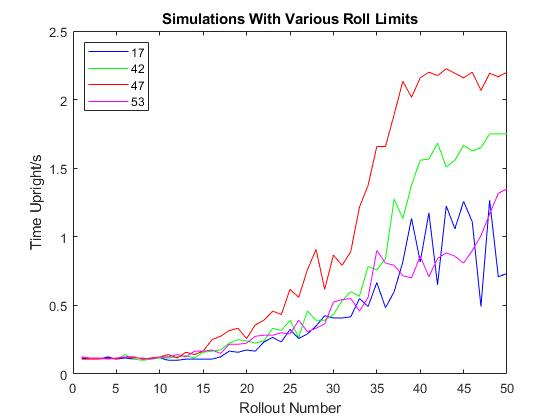
\includegraphics[width=\linewidth]{average_angle}
   \caption{Average of six tests}
  \label{fig:a}
  \end{subfigure}
  \begin{subfigure}[t]{0.325\textwidth}
    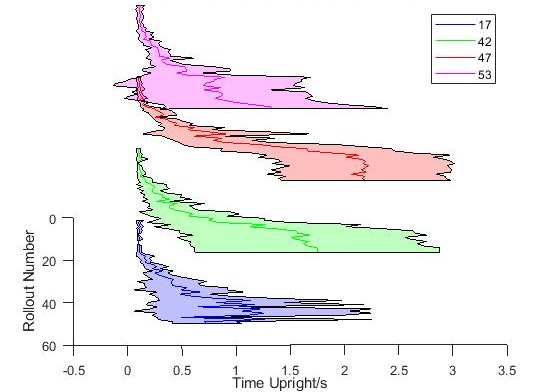
\includegraphics[width=\linewidth]{disp_angle}
    \caption{With $\pm \sigma$}
  \label{fig:sd}
  \end{subfigure}
  \begin{subfigure}[t]{0.325\textwidth}
    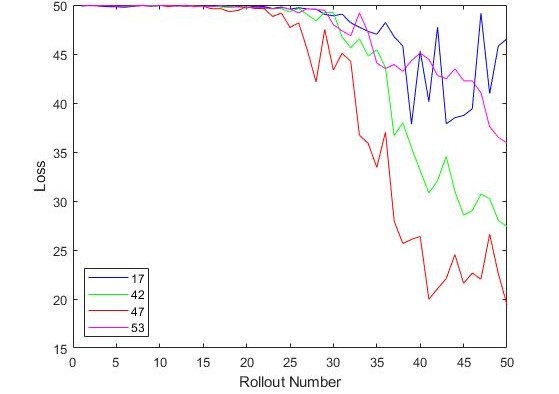
\includegraphics[width=\linewidth]{average_angle_loss}
    \caption{Comparing against rollout loss}
  \label{fig:rl}
  \end{subfigure}
  \caption{Simulating the effect of roll limit $\theta_{max}$ }
  \label{fig:rolllimit}
\end{figure*}
The first factor that would determine the benefit of a large mechanical redesign is the roll limit. In the unicycle model the roll angle cannot exceed 17 degrees. This is thought to inhibit learning as initially the system can't balance and will hit this limit within very few time steps. This could mean the model has insufficient data to successfully learn a policy. Furthermore as the last measurement is removed in real trials due to high accelerations the data available is reduced more. This reduction will have a larger effect on small roll limits and can cause failure to appear to happen at a low cost. Which could in turn inhibit learning more.
\newline
Several designs were sketched to change the roll limit. 42 degrees could be achieved with a new chassis and the same gears, and 47 degrees by changing an additional bracket. Simulations of these can be seen in figure \ref{fig:rolllimit}.
\newline
After 10 random rollouts the roll limit made little difference as in figure \ref{fig:a}. However, when policy optimisation started then a higher roll limit improved success greatly. The change between 42 and 47 degrees appears significant which shows more progress is likely to be made by increasing roll limit further. The plateau observed at 47 degress is due to some tests consistently staying upright for the whole horizon time. When looking at rollout total loss in figure \ref{fig:rl} the same pattern is observed with a higher roll limit reducing the overall rollout loss.
\newline
The variation between simulations can be seen in figure \ref{fig:sd} and shows greater reliability at higher roll limits, with a standard deviation of spread at 47 degrees close to being higher then the mean at 42 degrees. The spread is very important to create a reliable policy training method.
\newline
Higher roll limits could be achieved by changing other parts. 53 degrees would require a 5mm larger wheel. This change would require evaluating the effect wheel size had on performance as well as roll limit.


\begin{figure}[h]
  \centering
  \begin{subfigure}[t]{0.5\textwidth}
    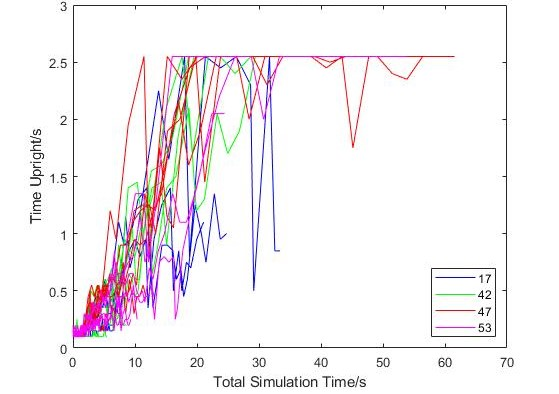
\includegraphics[width=\linewidth]{all_angle}
   \caption{Vary roll limit}
  \label{fig:wxro}
  \end{subfigure}
  \newline
  \begin{subfigure}[t]{0.5\textwidth}
    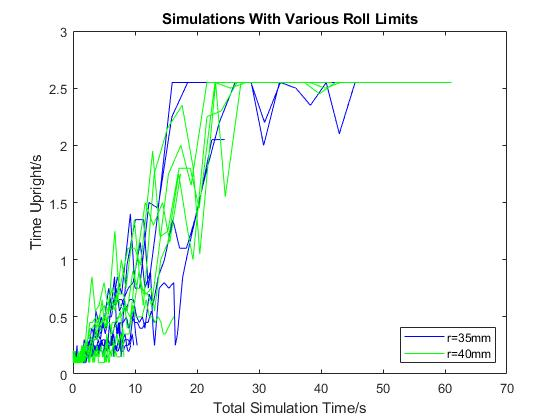
\includegraphics[width=\linewidth]{all_wheel}
    \caption{Vary wheel size}
  \label{fig:exwh}
  \end{subfigure}
  \caption{Simulated performance compared to experience time}
  \label{fig:exti}
\end{figure}
%-----------------------------------
\subsection{Sampling Time}
Sampling time is another important factor to consider when optimising the training situation of the real unicycle. A faster sampling time effects the following:

\begin{itemize}
\item Dynamics change slower and more linearly between readings, decreasing modelling complexity and improving predictions.
\item A zero order hold controller is used on the motors, with torque calculated at the start of a step. As the unicycle moves this action is non optimum, therefore an error is introduced.
\item More data points are collected, this can help build better models but at the expense extra computational time.
\item Every policy call injects noise into the predictions from process and measurement noise. This causes a more uncertain trajectory prediction over the horizon time.
\end{itemize}

Not enough tests have been simulated yet to fully determine the effect. However, new learning behaviours which prioritised distance to origin over just being upright were observed. Therefore showing promise that sampling time can greatly effect learning.

\begin{figure}[h]
  \centering
    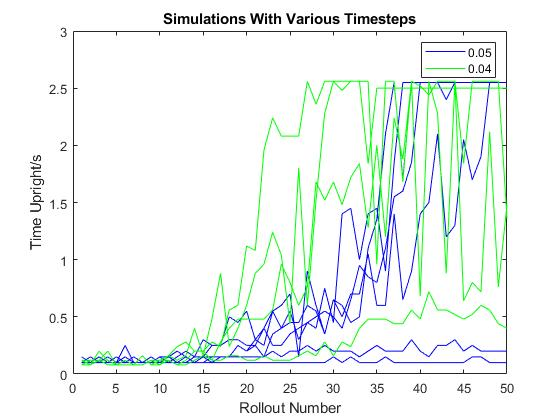
\includegraphics[width=\linewidth]{all_ts}
  \caption{Effect of sampling time change}
  \label{fig:st}
\end{figure}
Figure \ref{fig:st} shows the results of changing timestep for a roll limit of 42 degrees. Not enough tests have been conducted yet due to the increased simulation time meaning no conclusions can be drawn yet. The lower performing trial at 0.04s did show promise as it learnt to balance in a different way to all other trials, it prioritised staying at the origin over staying upright. This shows that there is a possibility of the timestep greatly effecting learning and should be pursued further.

%---------------------------------------------
\subsection{Wheel Size}
\begin{figure}[h]
  \centering
    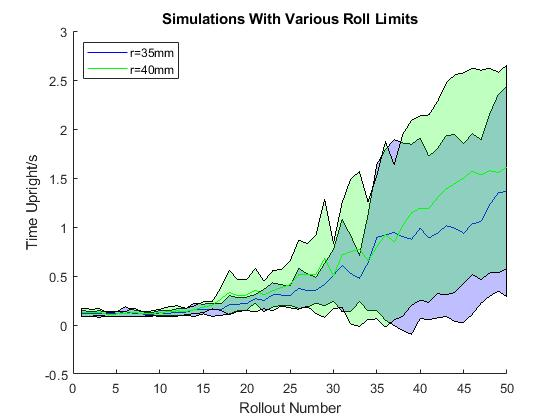
\includegraphics[width=\linewidth]{disp_wheel}
  \caption{Effect of wheel size when roll limit is 5=$53^{\circ}$}
  \label{fig:whellsi}
\end{figure}

%--------------------------------
\subsection{Future Simulations}
Additional factors are to be simulated to determine the variables that effect learning rate the most. These are the following:

\begin{itemize}
\item Higher roll limits with larger wheels.
\item More sampling times.
\item Strength of the cost function.
\item Motor torques.
\end{itemize}
%------------------------------------------------


%---------------------------------------
\clearpage
\begin{figure*}
\centering
\begin{subfigure}[t]{0.49\textwidth}
    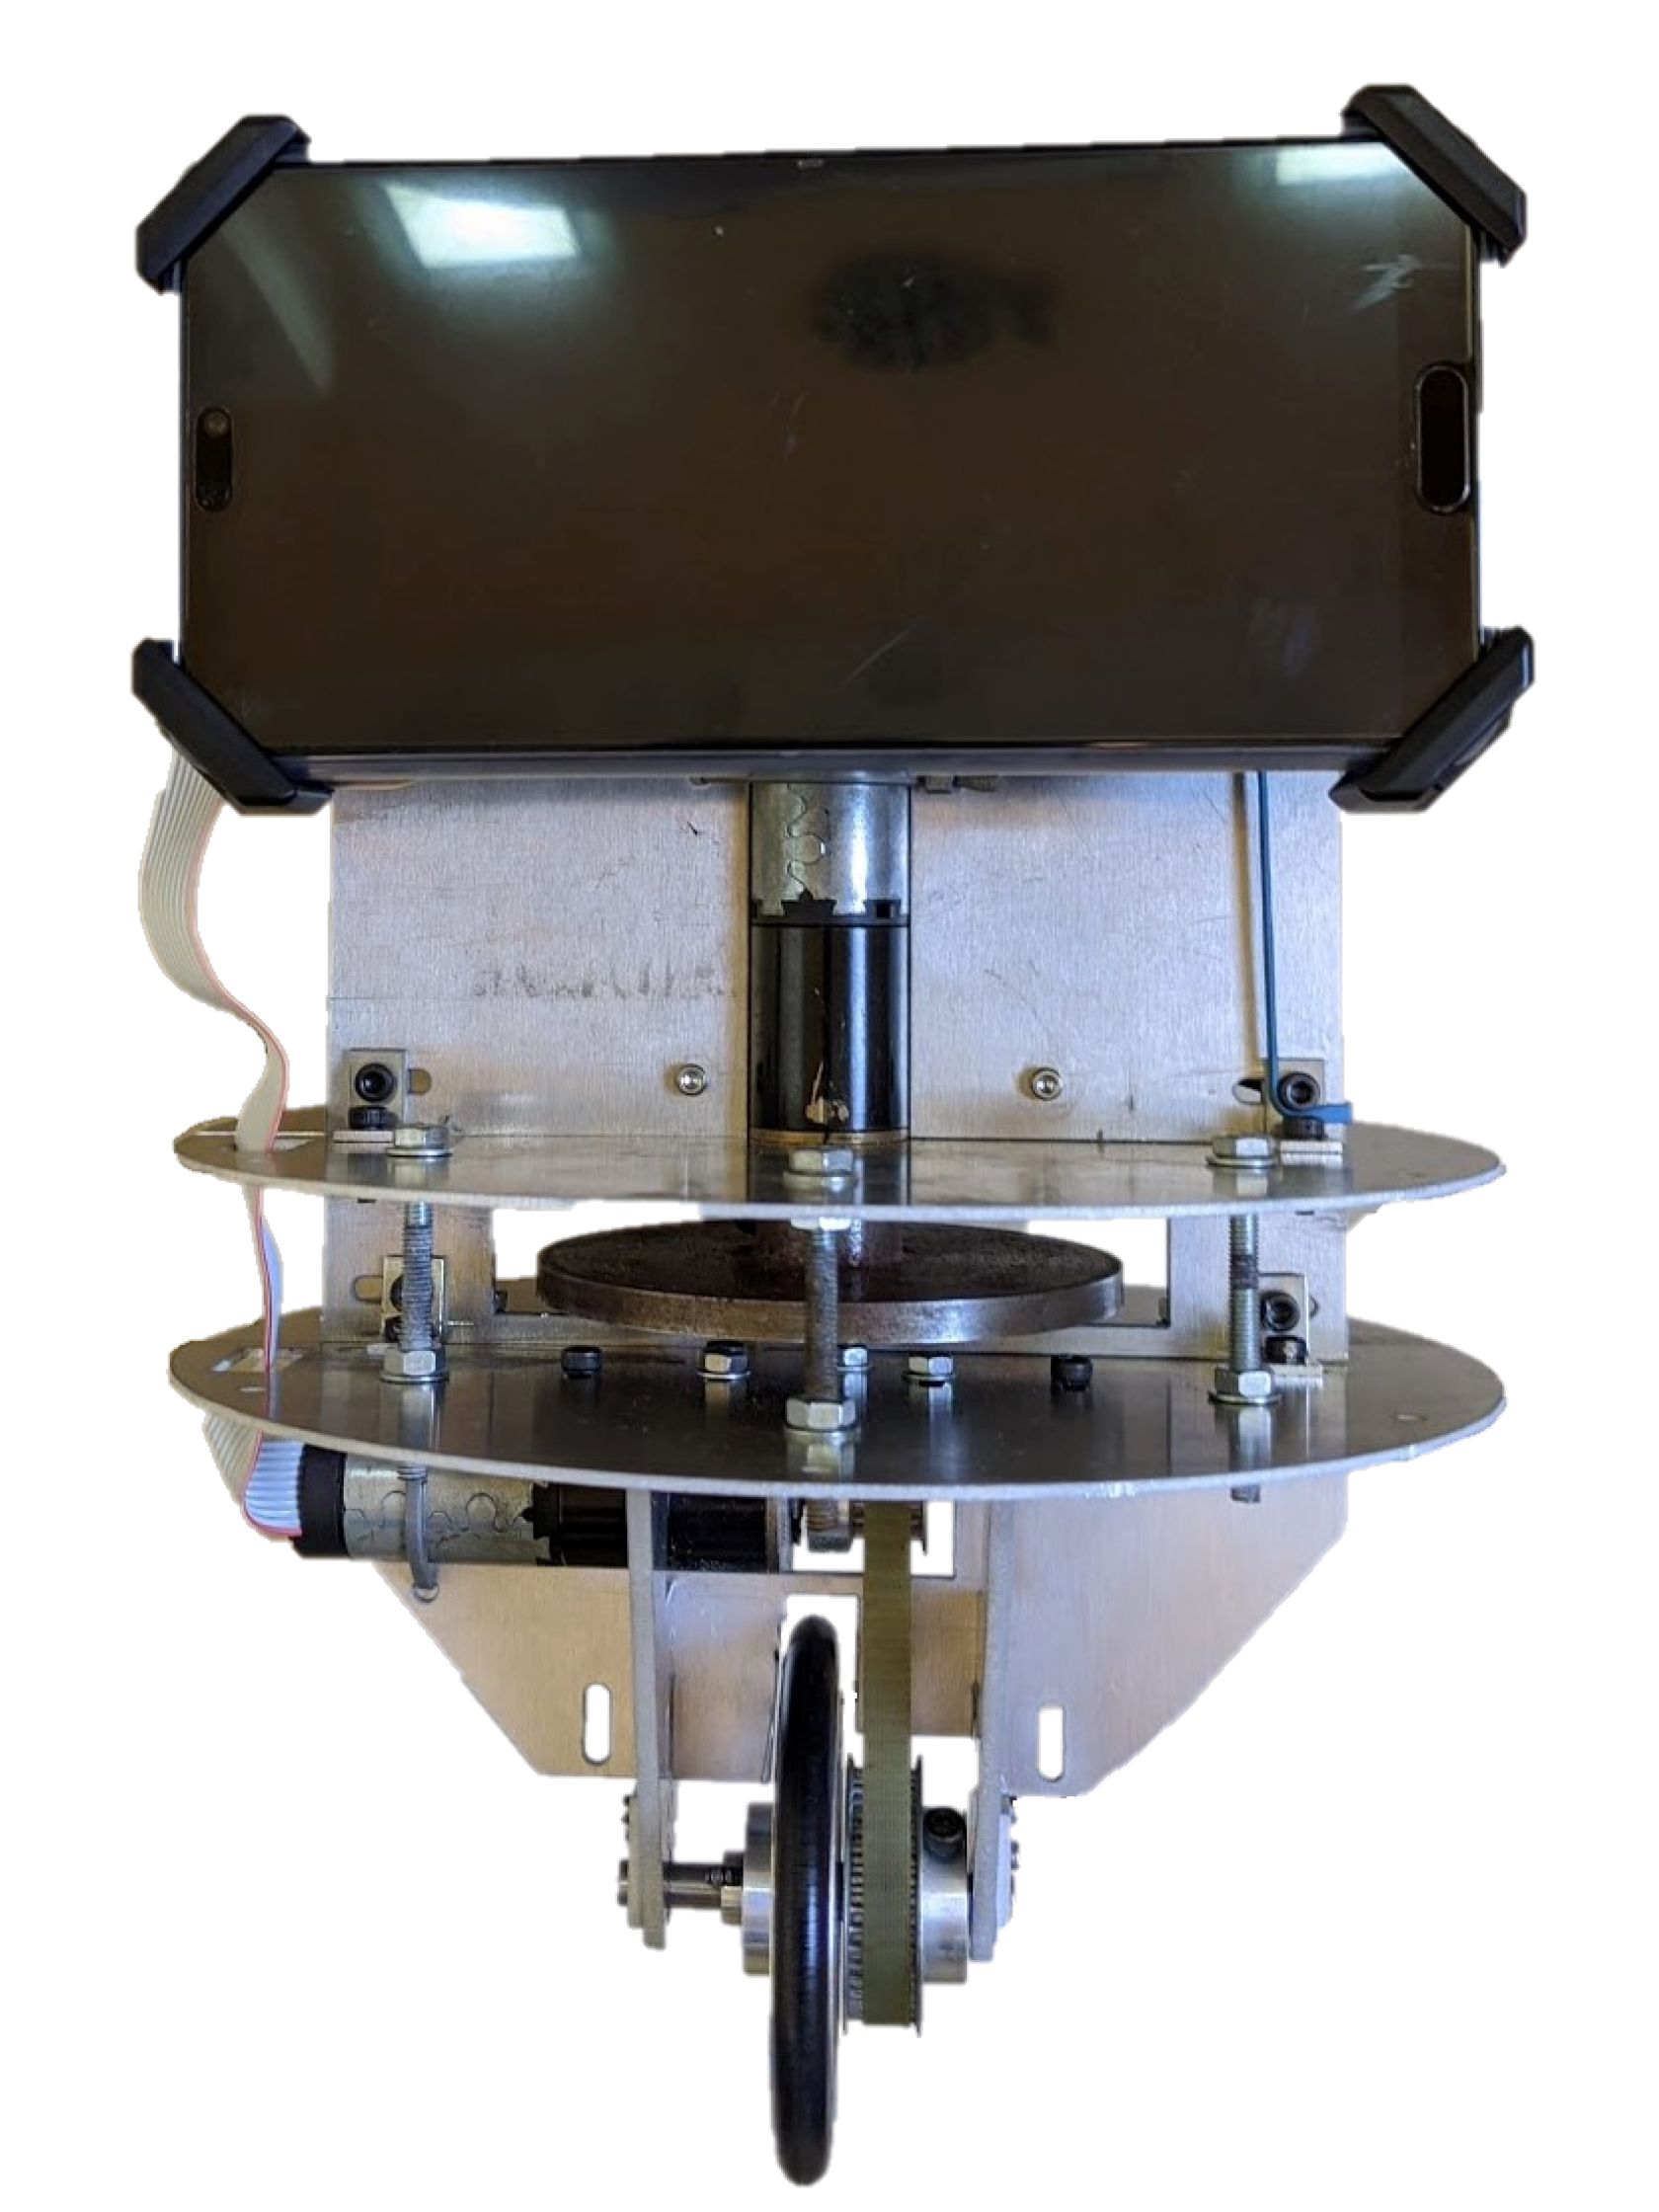
\includegraphics[width=\linewidth]{frontnewt}
   \caption{Front}
  \label{sub:frontnew}
  \end{subfigure}
  \begin{subfigure}[t]{0.49\textwidth}
    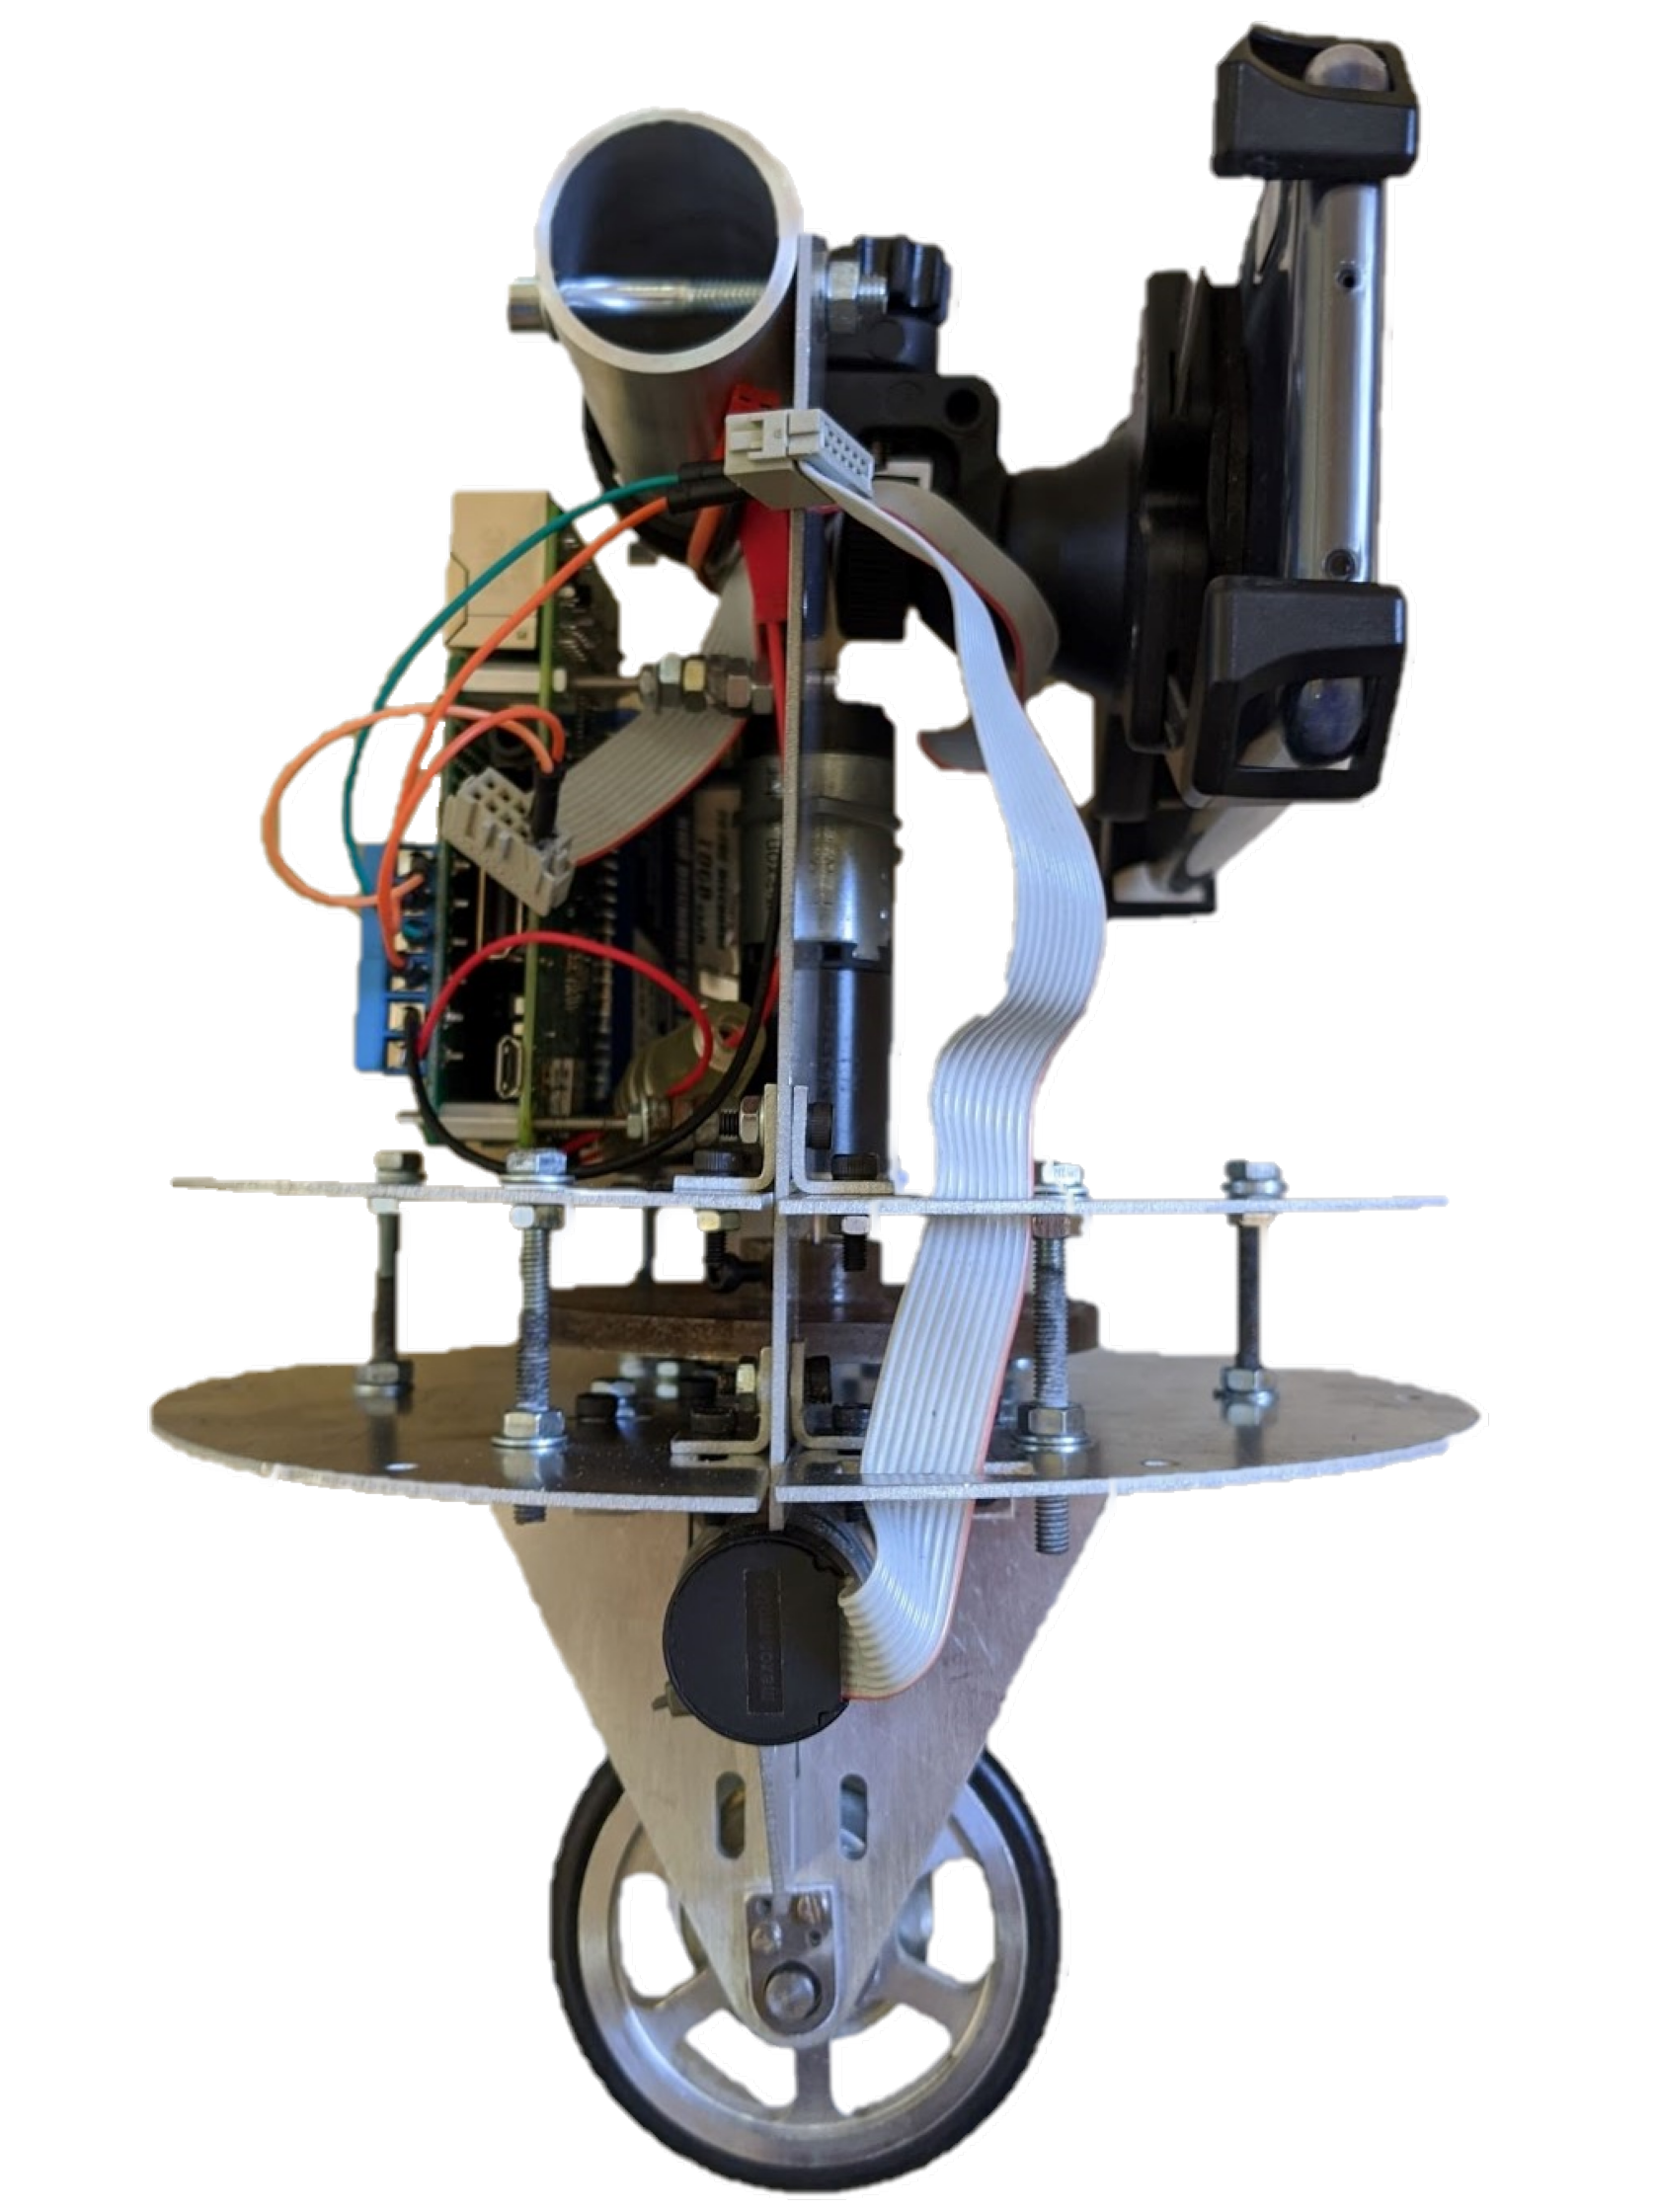
\includegraphics[width=\linewidth]{sidenewt}
    \caption{Side}
  \label{sub:sidenew}
  \end{subfigure}
  \newline



\tabskip=0pt
\valign{#\cr
  \hbox{%
    \begin{subfigure}[b]{.49\textwidth}
    \centering
    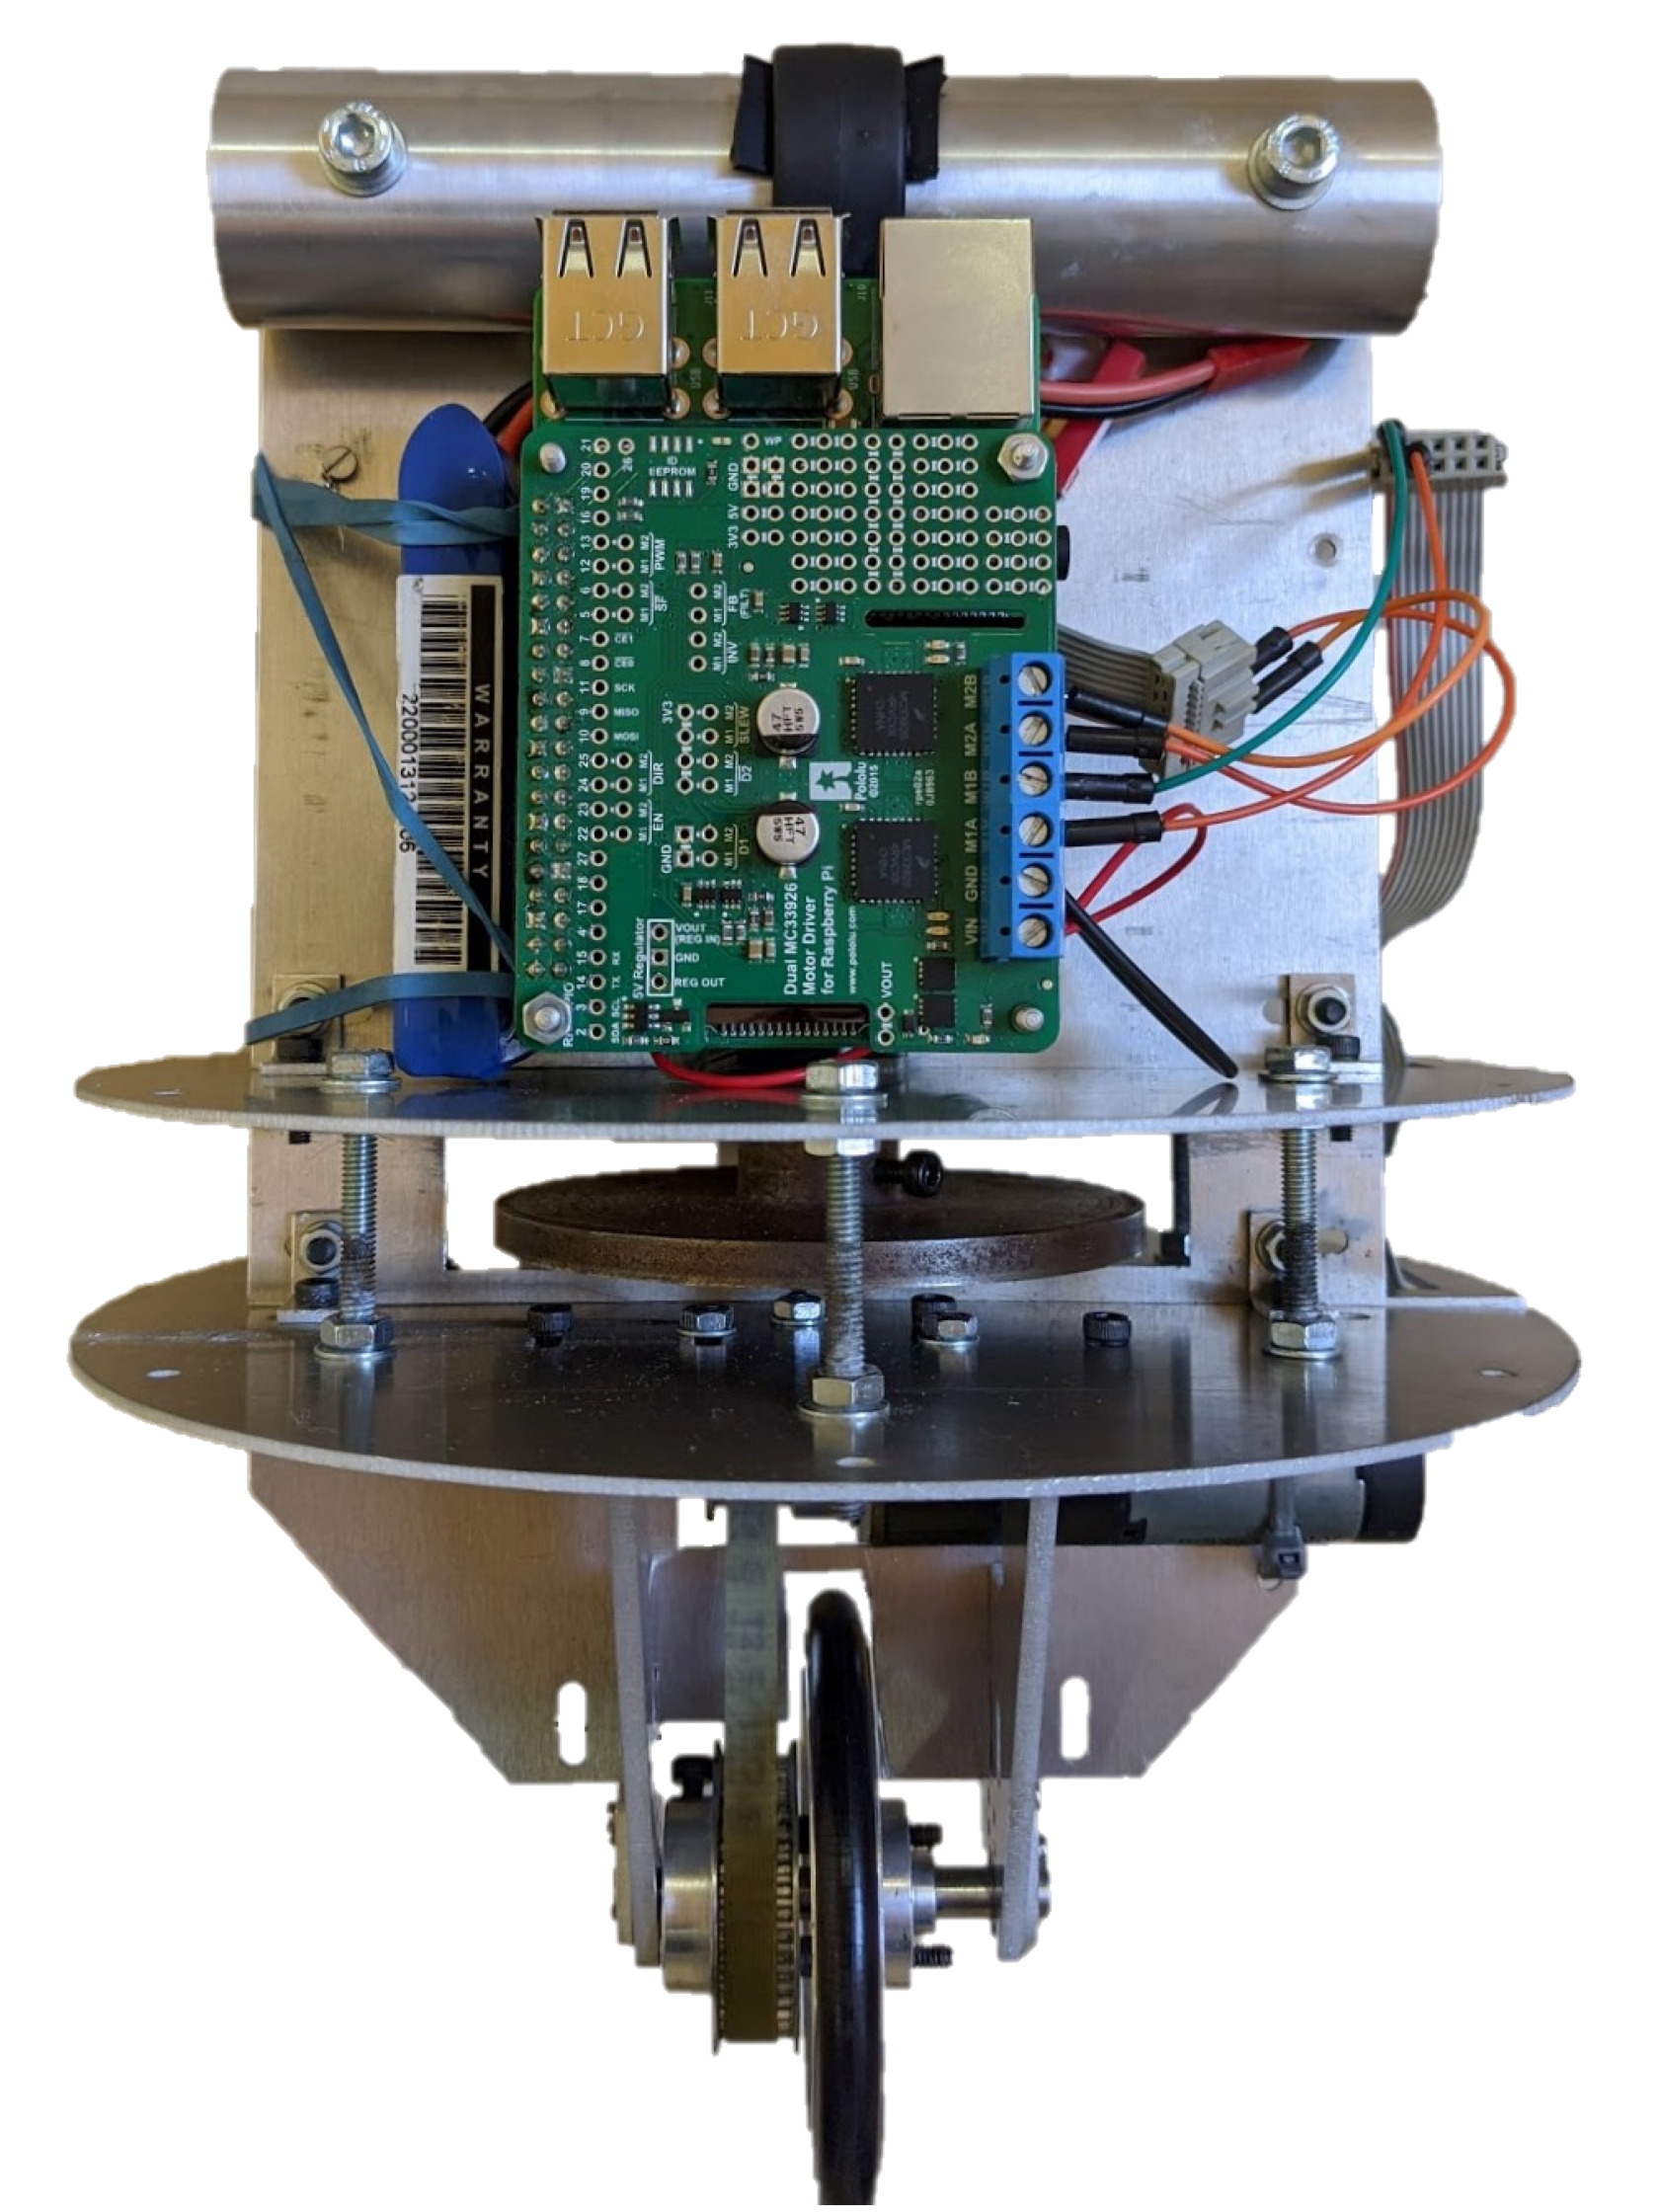
\includegraphics[width=\linewidth]{backnewt}
     \caption{Back}
  \label{sub:backnew}
    \end{subfigure}%
  }\cr
  \noalign{\hfill}
  \hbox{%
    \begin{subfigure}{.49\textwidth}
    \centering
    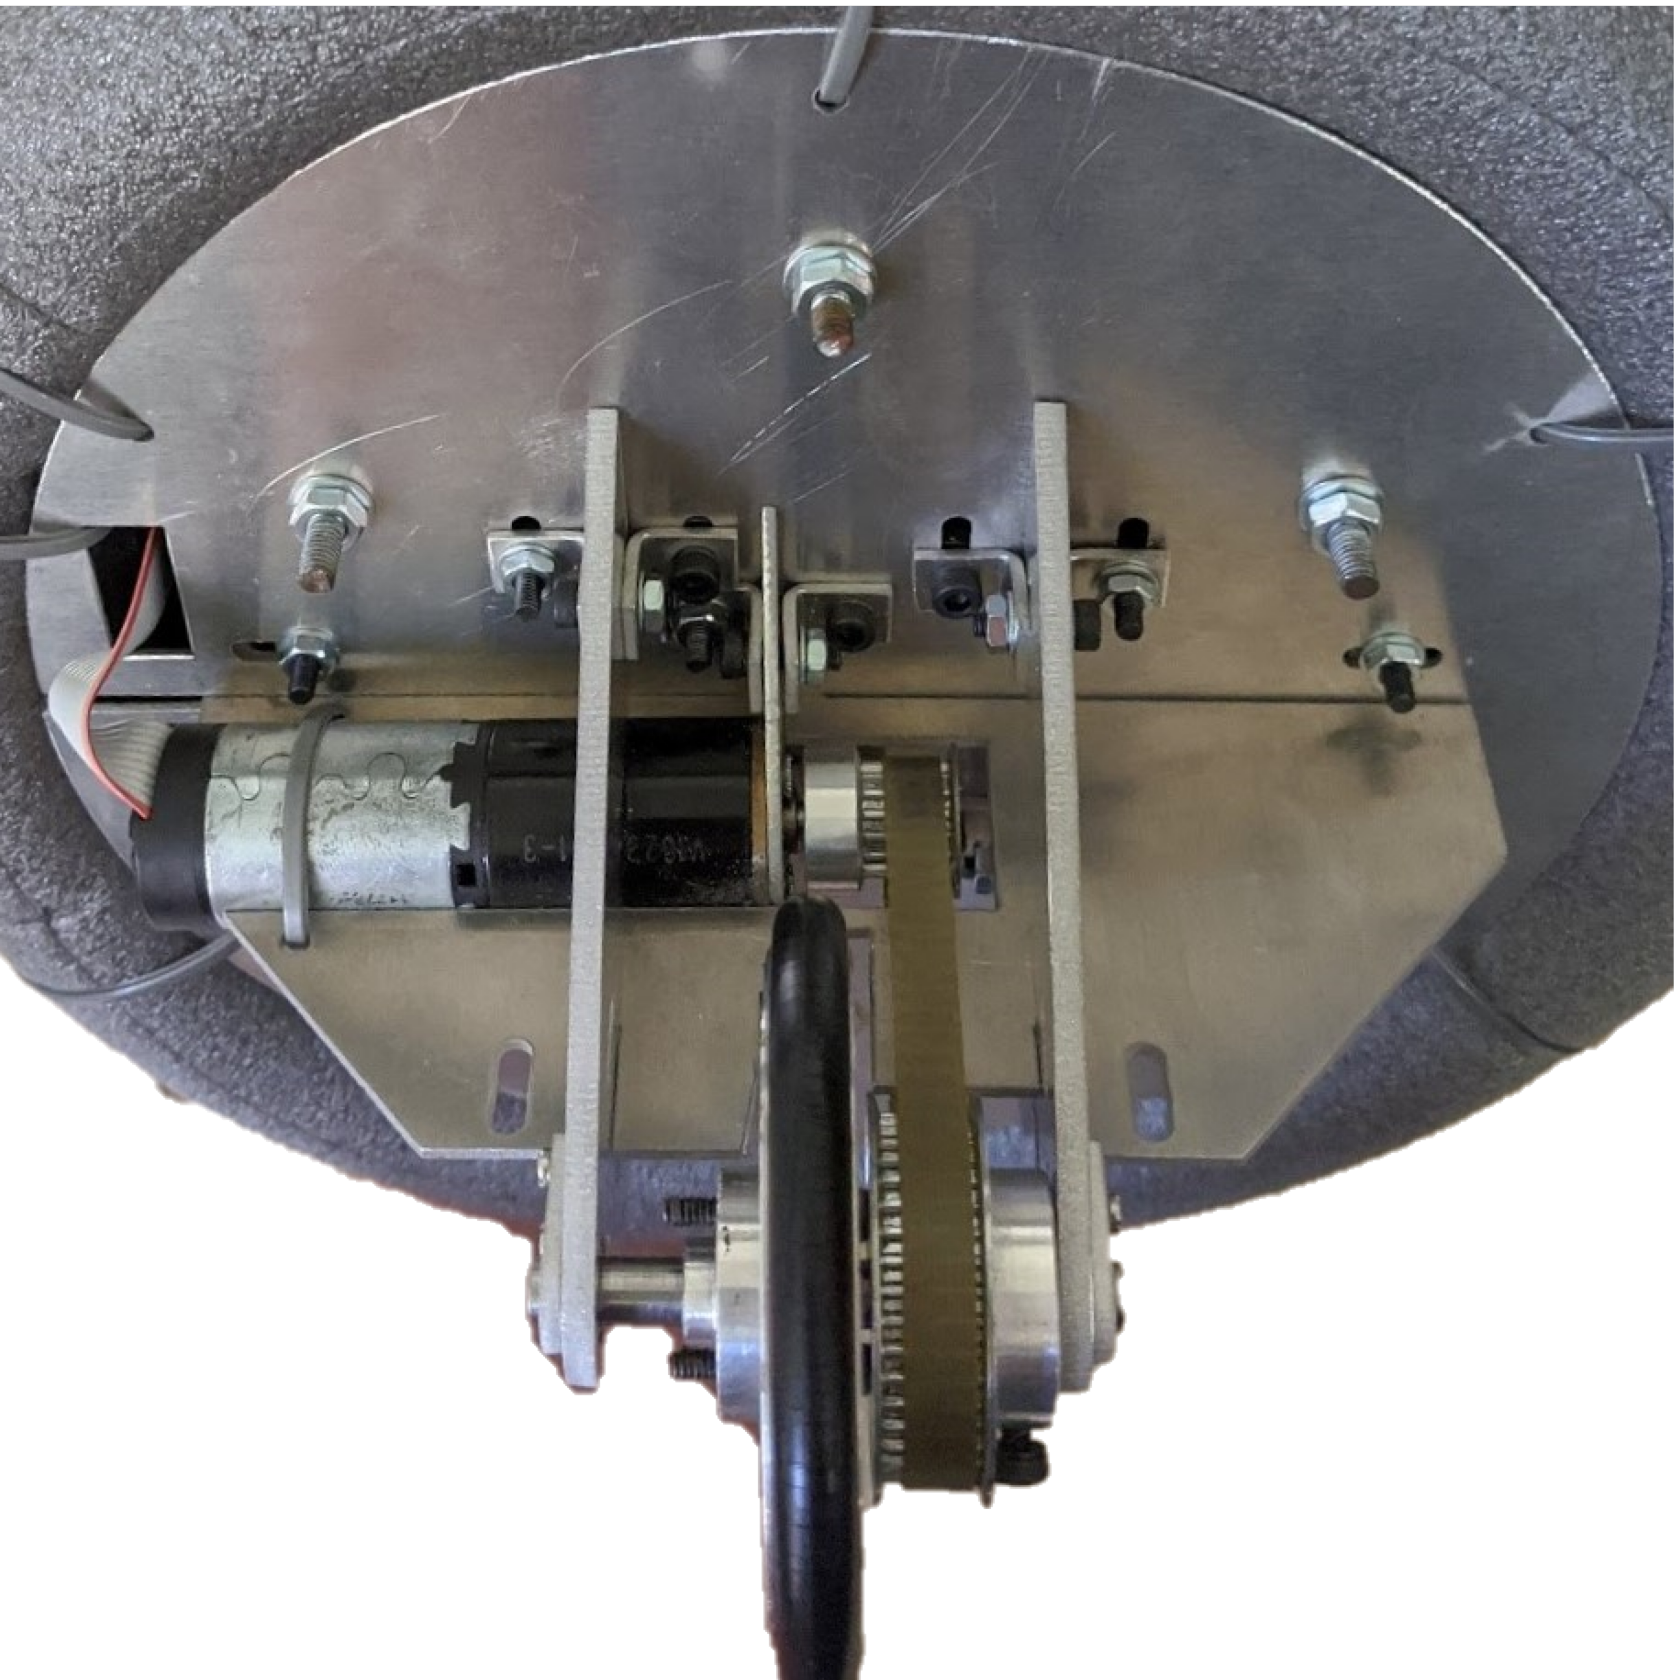
\includegraphics[width=.602\textwidth]{botnewt}
     \caption{Bottom}
  \label{sub:botnew}
    \end{subfigure}%
  }\vfill
  \hbox{%
    \begin{subfigure}{.49\textwidth}
    \centering
    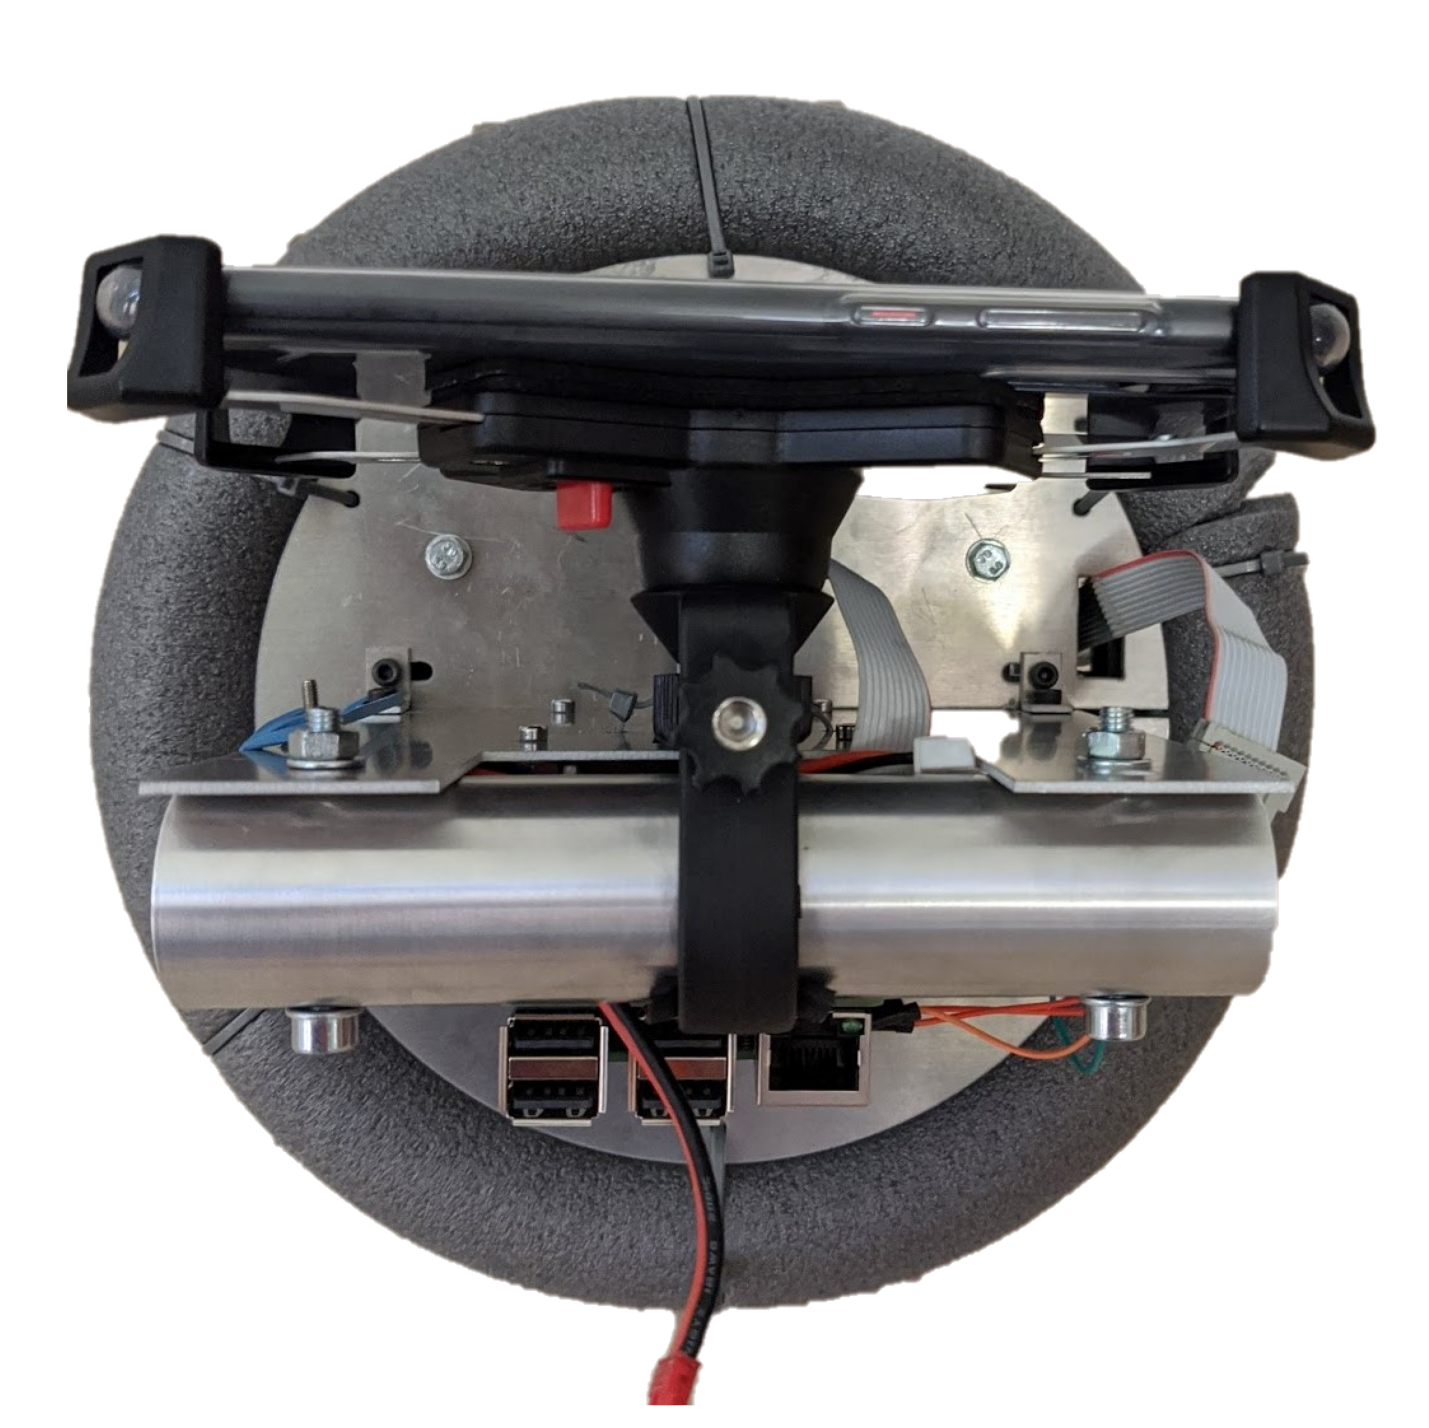
\includegraphics[width=.602\textwidth]{topnewt}
     \caption{Top}
  \label{sub:topnew}
    \end{subfigure}%
  }\cr
}

  \caption{New set-up of unicycle}
  \label{fig:new}
\end{figure*}





\begin{figure*}[t!]
  \centering
  \begin{subfigure}[t]{0.325\textwidth}
    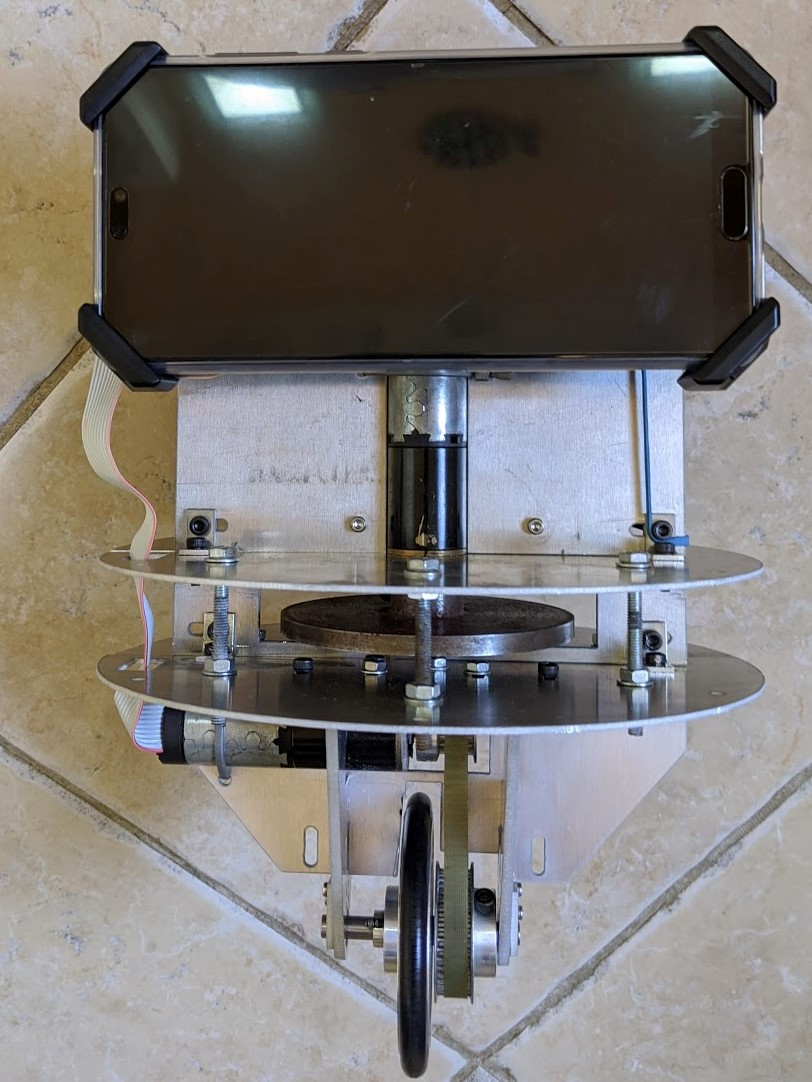
\includegraphics[width=\linewidth]{frontnew}
   \caption{Front}
  \label{sub:frontnew}
  \end{subfigure}
  \begin{subfigure}[t]{0.325\textwidth}
    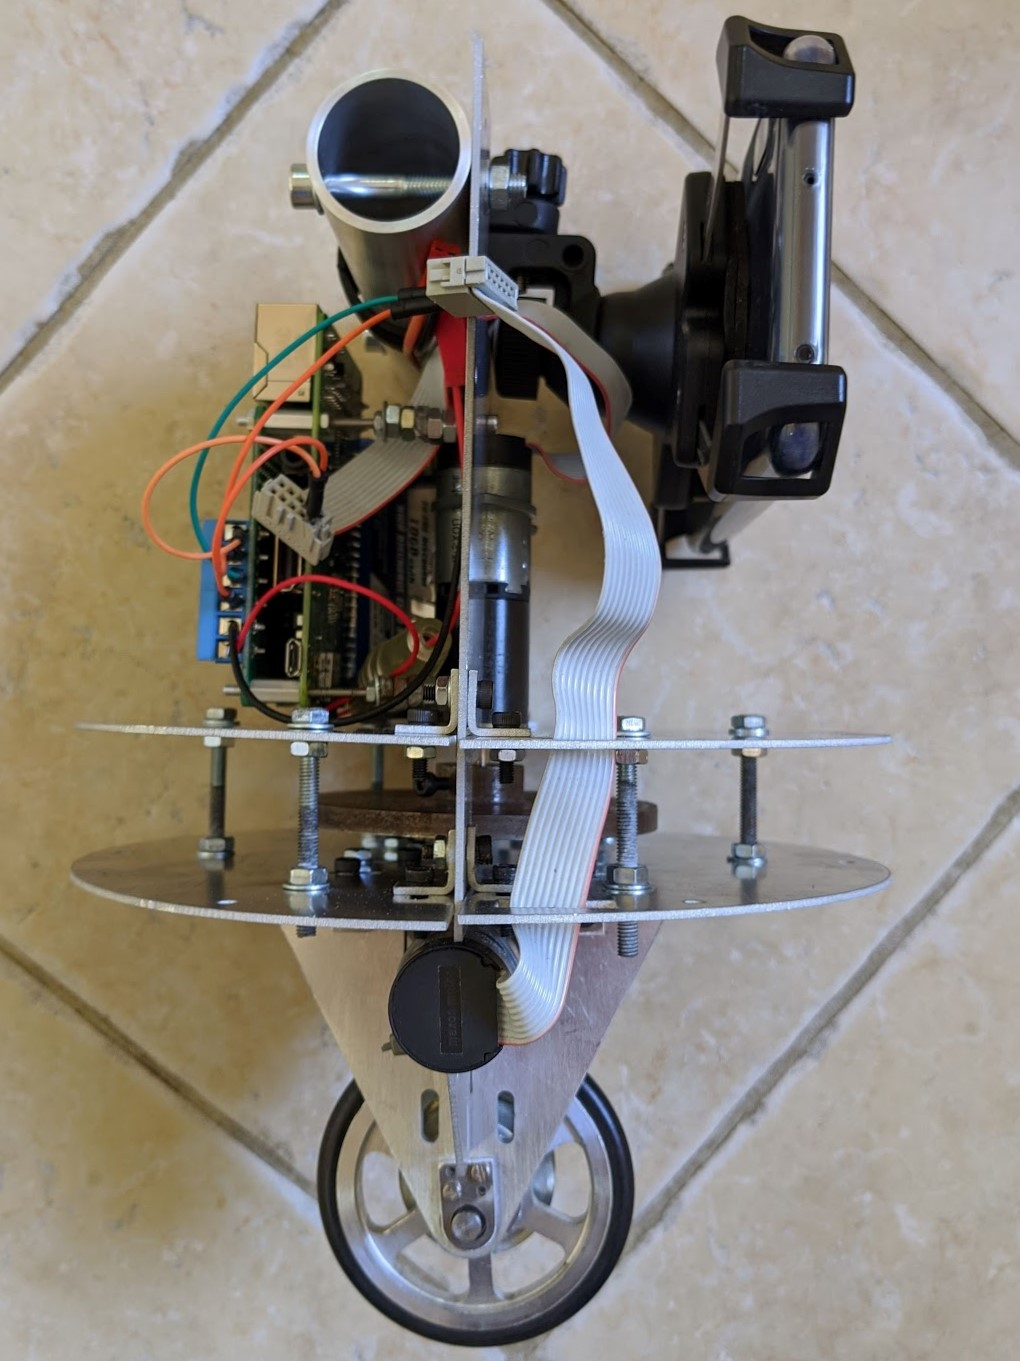
\includegraphics[width=\linewidth]{sidenew}
    \caption{Side}
  \label{sub:sidenew}
  \end{subfigure}
  \begin{subfigure}[t]{0.325\textwidth}
    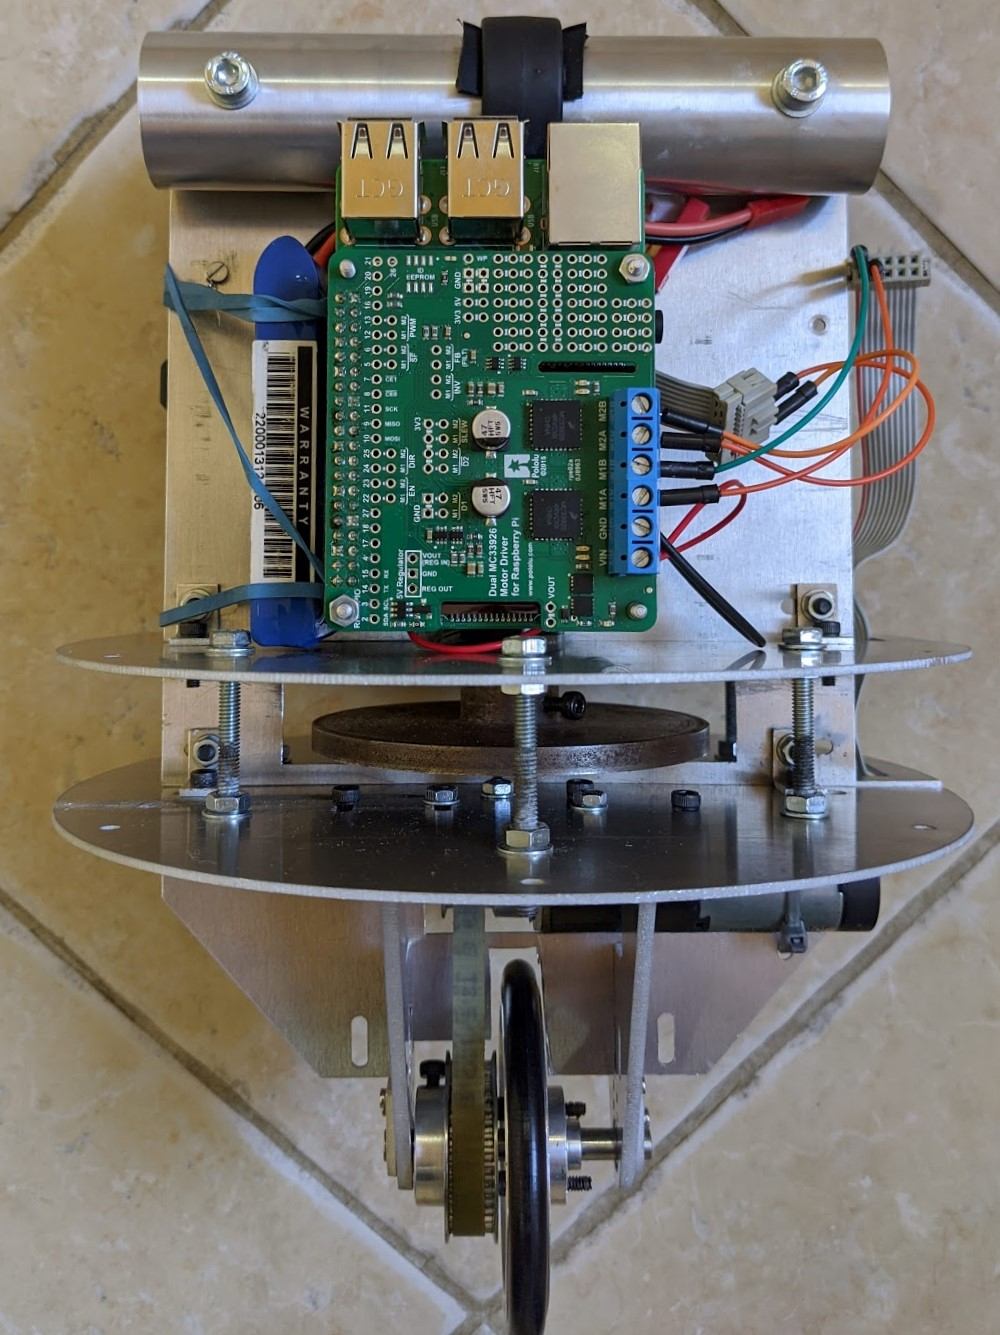
\includegraphics[width=\linewidth]{backnew}
    \caption{Back}
  \label{sub:backnew}
  \end{subfigure}
  \newline
  
  \begin{subfigure}[t]{0.325\textwidth}
    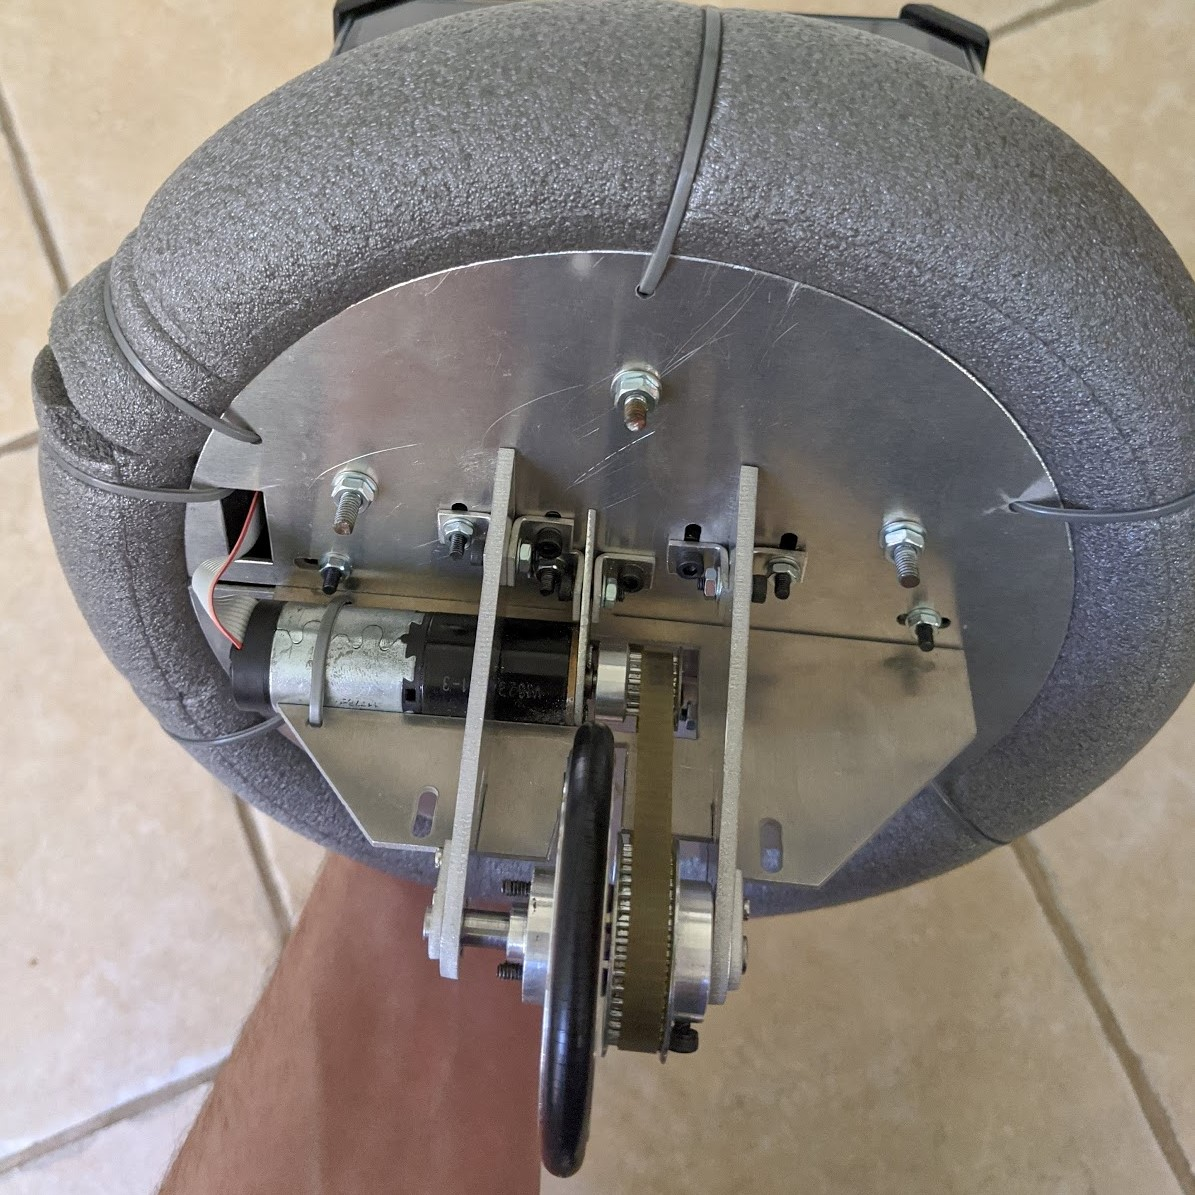
\includegraphics[width=\linewidth]{botnew}
    \caption{Bottom}
  \label{sub:botnew}
  \end{subfigure}
  \begin{subfigure}[t]{0.325\textwidth}
    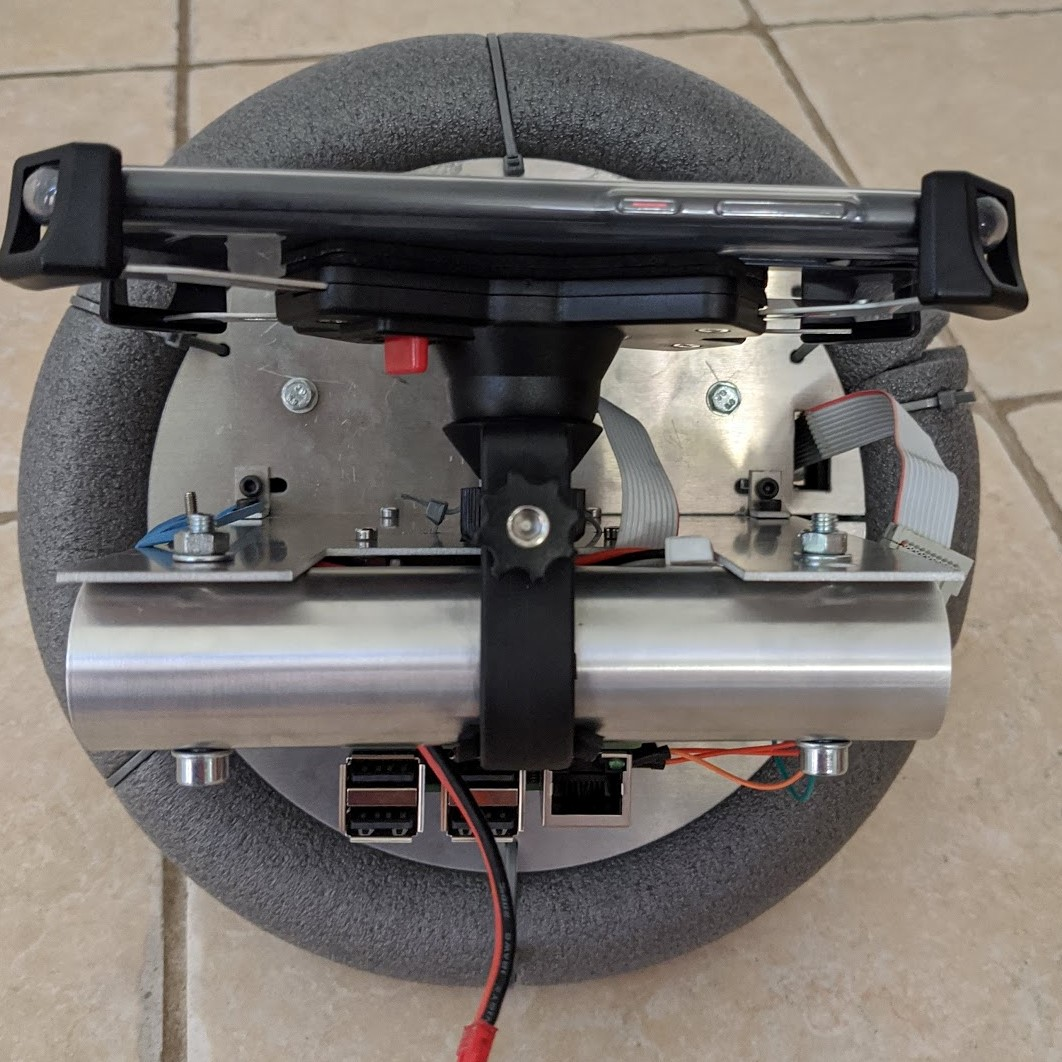
\includegraphics[width=\linewidth]{topnew}
    \caption{Top}
  \label{sub:topnew}
  \end{subfigure}
  
  \caption{Drawings of new unicycle design}
  \label{fig:drawings}
\end{figure*}
\clearpage
\section{Mechanical redesign}
Speculations from previous years and simulations results conducted indicated that the unicycle was unable to learn to balance with a roll limit of 17 degrees. This prompted the need for a new unicycle design pictured in figure \ref{fig:new} and \ref{fig:drawings}. In order to allow for a good design the following principles were adopted:

\begin{itemize}
\item Replace welding with bolts, to allow for easy part replacement if required in future
\item Maintain rigidity with the use of bolts
\item Keep parts as simple as possible
\item Allow for variation in parts eg phone size
\end{itemize}

\subsection{Changes}
\subsubsection{Roll limit}
From simulations it was shown that increasing the roll limit to $47^{\circ}$ was required to allow policy learning. Increasing the limit much further simulations deemed unnecessary.

\begin{figure}
  \centering
    
\includegraphics[width=\linewidth]{place}
  \caption{New design for higher roll limit}
  \label{fig:newline}
\end{figure}

Figure \ref{fig:newline} shows a comparison between the old $17^{\circ}$ design and new $47^{\circ}$ design. This was made possible using mostly the same parts from the original design, with the exception of bearings. This was to maintain the gear ratio shown to be effective, and to reduces the need to source new parts that would make very marginal differences. 
\newline
The first step to increasing roll limit was to bring the gears and motors as central as possible. This required decentralising the motor position and therefore CoM. The unicycle should still be able to learn with an off-centre design, however this would still be corrected for with later part placement. Once all the parts had been centralised it was found that the roll limit was $42^{\circ}$ with the axle bracket the limiting factor. 
\newline
Three steps were implemented to reduce this limit. Reduce size of bearing holder, use smaller 10x6mm bearing, and minimise size of axle mount. These changes allowed the roll limit to become $47^{\circ}$ as desired.
%--------------------------------------
\begin{table*}[ht!]
\centering
\begin{tabular}{ c | c | c | c }
Design& Summary & USB-C & Total\\ 
\midrule
1&&1.05 &3.02\\
2&& 1.26&1.25\\
3&&1.02 &1.84\\
\end{tabular}
\caption{Protection system analysis}
\label{tab:pro}
\end{table*}

\subsubsection{Protection}
The next problem to solve was protecting the unicycle was the many falls it would experience. To be effective this would need to decelerate the unicycle at a slow rate, be easy to attach and fix if damaged, be mounted to not decrease the roll limit by too much.
\newline
Three designs were proposed an evaluation of which can be seen in table \ref{tab:pro}. Design 1 consisted of a static material eg rubber or foam being attached, design 2 was a large ring attached to the main chassis by springs, and design 3 was an inflated inner tube. The design that proved to be the most effective at achieving the initial aims was a static material damper. This was due to its simplicity and ease of replacement, while still maintaining effectiveness. To decide the material various items were tested by hand. These were rubber tubing, foam insulation tubing, hose pipes, silicon seals. Out of these materials only the foam tubing was the desired stiffness and thickness for the task. The tubing came with the added benefit of being the cheapest and has the option to increase stiffness if required by threading extra material inside it.

\begin{equation}
d = 
\label{eq:diskdia}
\end{equation}

The foam was to be mounted to the horizontal metal disks protecting the flywheel. A roll limit of $45^{\circ}$ was designed for the point of contact on the tube allowing for $2^{\circ}$ of deceleration to occur. This corresponded to a displacement of ....... in the foam. The required disk diameter for mounting was calculated using equation \ref{eq:diskdia}. Where t=26mm is the disk separation, and r=15mm is the foam radius.

%--------------------------------------
\subsubsection{Mountings}
The previous method of mounting the phone used elastic bands. This resulted in lengthy repositioning of the phone between trials to minimise the cross trial effect of sensor position change. This introduces a lot of avoidable noise if done incorrectly. The aim was to decrease this variation by providing a secure mounting that was capable of fixing any phone, in case this changed in the future. 
\newline
To have reliable and repeatable phone position the attachment must resisting all degrees of freedom and have at least 3 reference planes f phone alignment. Due to these strict requirements and desire for size variability it was decided to use an existing phone mounting system. This would increase part size, but provide the desired functionality without need to fabricate complicated parts. Different bike and car mounts were evaluated with the ...... bike mount eventually chosen \cite{bike}. This mounts onto a handlebar like design at the top of the unicycle as in figure \ref{sub:topnew}. 
\newline
The Raspberry Pi was attached using long bolts located on the opposite side to the phone. In addition to the battery these were located slightly off centre, see figure \ref{sub:backnew}. This countered the off centred motor position for the wheel, and successfully brought the CoM to the centre. The Pi was located further away from the central plane of the unicycle then desired, this was due to the inability to find suitably shorter screws, and spacers because of closures due to Covid-19. By shortening these screws the moment of inertia would reduce and could improve unicycle balance.  
%--------------------------------------
\subsubsection{Material}
A copper coated fibre glass was used previously, as it had high stiffness but low weight. Due to designing within solidworks and requiring some machined parts the EDG office who manufactured the parts last time were unable to help again. Therefore a change in material was required to 1.6mm plate aluminium, with the manufacturing done in the Dyson centre workshop. This ensured that the frame would be stiff enough to limit unwanted vibrations without adding too much weight. 
\subsection{Inertia}
\begin{table*}[ht!]
\centering
\begin{tabular}{ c | c | c | c | c | c | c | c | c | c | c }
&  & &  &  & \multicolumn{3}{c|}{About CoM} & \multicolumn{3}{c}{About ground}\\
&  & &  &  & \multicolumn{3}{c|}{/ x$10^{-5kgm^2}$} & \multicolumn{3}{c}{/ x$10^{-3}kgm^2$}\\
Part& Mass/kg & x/m & y/m & z/m & $I_{xx}$ & $I_{yy}$  & $I_{zz}$ & $I_{xx}$ & $I_{yy}$  & $I_{zz}$ \\ 
\midrule
Phone & 0.2 & 0.06 & 0.7 & 0.2 & 46 & 8 & 38 & 8.5 & 8.7 & 1.0\\
Back Plate & 0.12 & 0 & 0 & 0.12 & 60 & 40 & 20 & 2.3 & 2.1 & 20\\
Disks & 0.1 & 0 & 0 & 0.11 & 19 & 19 & 38 & 2.8 & 2.8 & 0.76\\
Bot Motor & 0.12 & 0 & 0 & 0.09 & 4.6 & 0.7 & 4.6 & 1.0 & 1.0 & 0.05\\
Top Motor & 0.12 & 0 & 0 & 0.15 & 4.6 & 4.6 & 0.7 & 2.7 & 2.7 & 0\\
Axel support & 0.02 & 0 & 0.02 & 0.07 & 0.46 & 2.3 & 1.8 & 0.2 & 0.2 & 0.05\\
Flywheel & 0.2 & 0 & 0 & 0.11 & 8.1 & 8.1 & 16 & 2.5 & 2.5 & 0.16\\
Pi + battery & 0.15 & 0.04& 0 & 0.16 & 14 & 8 & 6 & 4.0 & 4.0 & 0.3\\
Handlebar & 0.067 & 0.015 & 0 & 0.22 & 1.3 & 12 & 1.3 & 3.2 & 3.3 & 0.3\\
Phone holder & 0.1 & 0.02 & 0 & 0.21 & 4.2 & 2.1 & 2.1 & 4.5 & 4.5 & 0.06\\
\midrule
\textbf{Total}
 &  & &  & 
 &  &  &  & 31.7 & 32.1 & 2.64\\
\end{tabular}
\caption{Moment of Inertia estimate}
\label{tab:mot}
\end{table*}

Table \ref{tab:mot} shows a rough estimation of the moment of inertia of the new unicycle about the group contact point. The estimations involved approximating each part to be a simple object such as planes, disks or cylinders. The using the formula from the mechanics data book the inertia about each parts CoM could be calculated and move by the parallel axis theorem to the contact point. The estimated inertias are 31.7, 32.1 and 2.64 $10^{-3}kgm^2$  for the x,y and z axis respectively. The inertia about the x and y axis are very similar as desired, meaning the unicycle should fall more uniformly in all directions. An estimation on the old unicycle was conducted for $I_{zz}$ \cite{arselan}, Harris assumed the unicycle was a cylinder and then checked his answer using measured angular accelerations. The value Harris calculated was 2.54$x10^{-3}kgm^2$ which is very similar to the new unicycle model.
\newline
The inertia about the vertical z axis is 16.4 times that of the flywheel. this means that to conserve angular momentum the flywheel needs to spin this much faster then the maximum rate of change in yaw. The motor has a maximum load speed of 3550rpm, after the 14:1 planetary gear this corresponds to a maximum angular speed of 26.5rad$s^{-1}$. Therefore a correction in yaw of up to 1.6rad$s^{-1}$ or a quarter rotation is expected. This speed seems high enough to enable learning.
\begin{equation}
\begin{split}
T = mgl sin\theta = I\ddot{\theta} \\
\ddot{\theta} = \frac{mgl}{I}sin\theta\\
dot{\theta} = \frac{mgl}{I}sin\theta t + c_1\\
\theta = \frac{mgl}{2I}sin\theta t^2 + c_1t + c_2\\
t = \sqrt{\frac{2\theta I}{mglsin\theta}} \\
\end{split}
\label{eq:rollt}
\end{equation}
The time required for the unicycle to fall without the motor input can be calculated using equations \ref{eq:rollt}. At t=0, $\dot{\theta}$ and $\theta$ = 0. This means that both constants are 0. By assuming the CoM is at l=0.16m and m=1.5kg the time to fall $45^{\circ}$ is calculated to be 1.2 seconds. However, from measuring the unicycle fall this time in reality is nearer to 0.6s. This reduction in time by half is caused by the wheel rolling as the motors were off, therefore reducing I as rotation no longer occurs about the contact point as assumed. While still present during rollouts this change will be less severe as the motors being powered stops them moving freely. This means a falling time between 0.6-1.2s is expected. With a timestep of 50ms this allows 12-24 recordings and commands to be present, even in bad rollouts. This is a large improvement on the last unicycle model which regularly saw around 3 readings before the $17^{\circ}$limit was reached.

%--------------------------------------
\subsection{Design Evaluation}
While constructing the unicycle it was apparent that the new design was more rigid and adaptable then the last model. Having the flywheel protection disks made out of one piece, instead of two welded together was the main source of this additional strength. The addition of the bolts also made assembling the model much easier which is promising if future modifications are needed. The most difficult part of assembly was securely attaching the top motor, this was due to the inaccessibility of the screws mounting it. This process was still easier then the last model as ample room had been made to remove the flywheel when the motors attached, allowing more room for tools. Some bolts are currently missing due to the inability to acquire more during the lockdown period of Covid-19. The addition of these bolts and ensuring all bolts are attached tightly is very important for minimising vibrational noise in future test runs.
\newline
The attachment of the Pi and phone proved very successful, allowing access to all the ports on both devices. The handle bar was a secure way of attachment and allowed for adequate variation in either phone orientation or size. Due to the mounting towards the top of the unicycle the moment of inertia about the wheel when falling is increased. This doesn't appear to be adversely affecting the unicycle performance as falling isn't happening too fast to react to. To improve this in future when the department is back open, weight could be removed from the inside of the handle bar, or mounting holes could possibly be moved lower down the back plate. This movement would also reduce the vibrations carried up this plate, which add unwanted noise to the sensor readings. Once again this problem doesn't appear to be too large and much easier methods of reduction could be implemented such as stiffeners attached to the plate edges.
\newline
The foam protection ring proved to be very effective. Roll angle was only marginally reduced as calculated, and the unicycle is able to safely fall without supervision. This part can easily be replaced by simply buying a new tube \cite{foam} and 7 cable ties.
\newline
Due to a change in material and slightly increase in size the overall weight of the unicycle was increased from 1.2kg to 1.5kg.. Inertia calculations and conducted rollouts show that the increase in weight and inertial still allows for good performance. However, if this proved problematic the easiest change would be to introduce a larger flywheel as there is room in the casing, or reposition the phone mounting. A larger flywheel would help increase yaw and roll adjustments, and moving the phone would reduce the largest contributor to $I_{xx},I_{yy}$ and therefore decrease topple speed.  

%--------------------------------------

%--------------------------------
\clearpage
\section{Results}
\subsection{Phone}
\subsubsection{Connection}
Previously the phone connected to the Matlab scrip on the computer using Matlab mobile and wifi. However, this feature has since been removed from Matlab mobile and delays caused by using wifi were believed to occur occasionally. This could introduce extra noise and incorrect state measurements decreasing learning ability.
\newline
HyperIMU \cite{ianovir} was used to replace Matlab mobile. This allowed connection using wifi and USB. The transmission protocol followed was UDP using the packet layout:

\begin{figure*}[t]
  \centering
  \begin{subfigure}[t]{0.325\textwidth}
    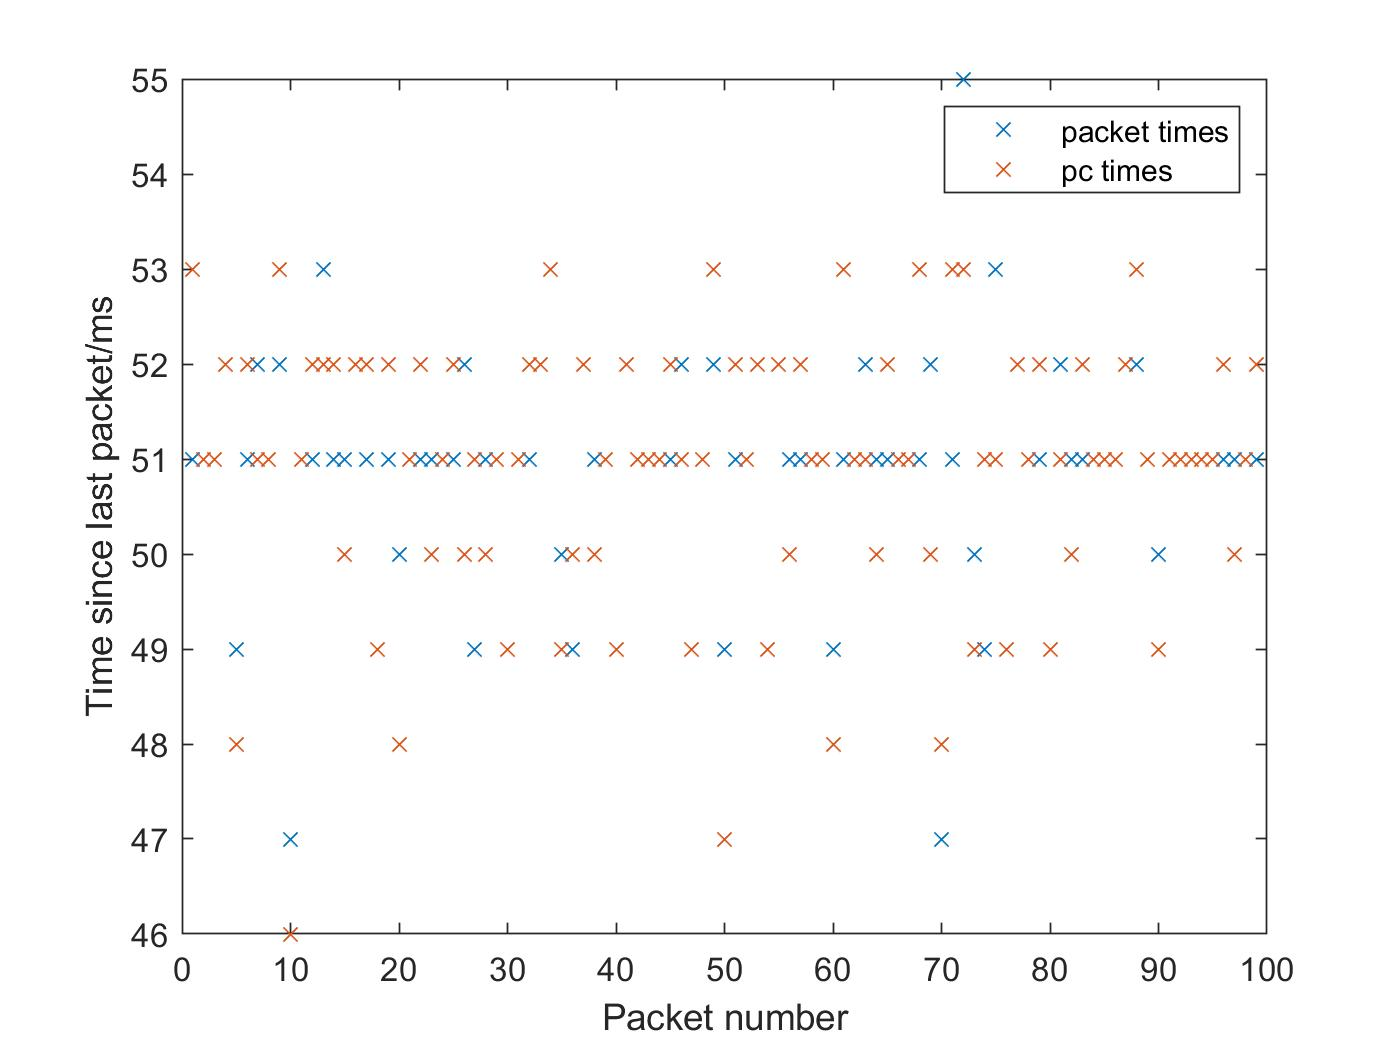
\includegraphics[width=\linewidth]{timestep}
   \caption{Time between measurements}
  \label{fig:ts}
  \end{subfigure}
  \begin{subfigure}[t]{0.325\textwidth}
    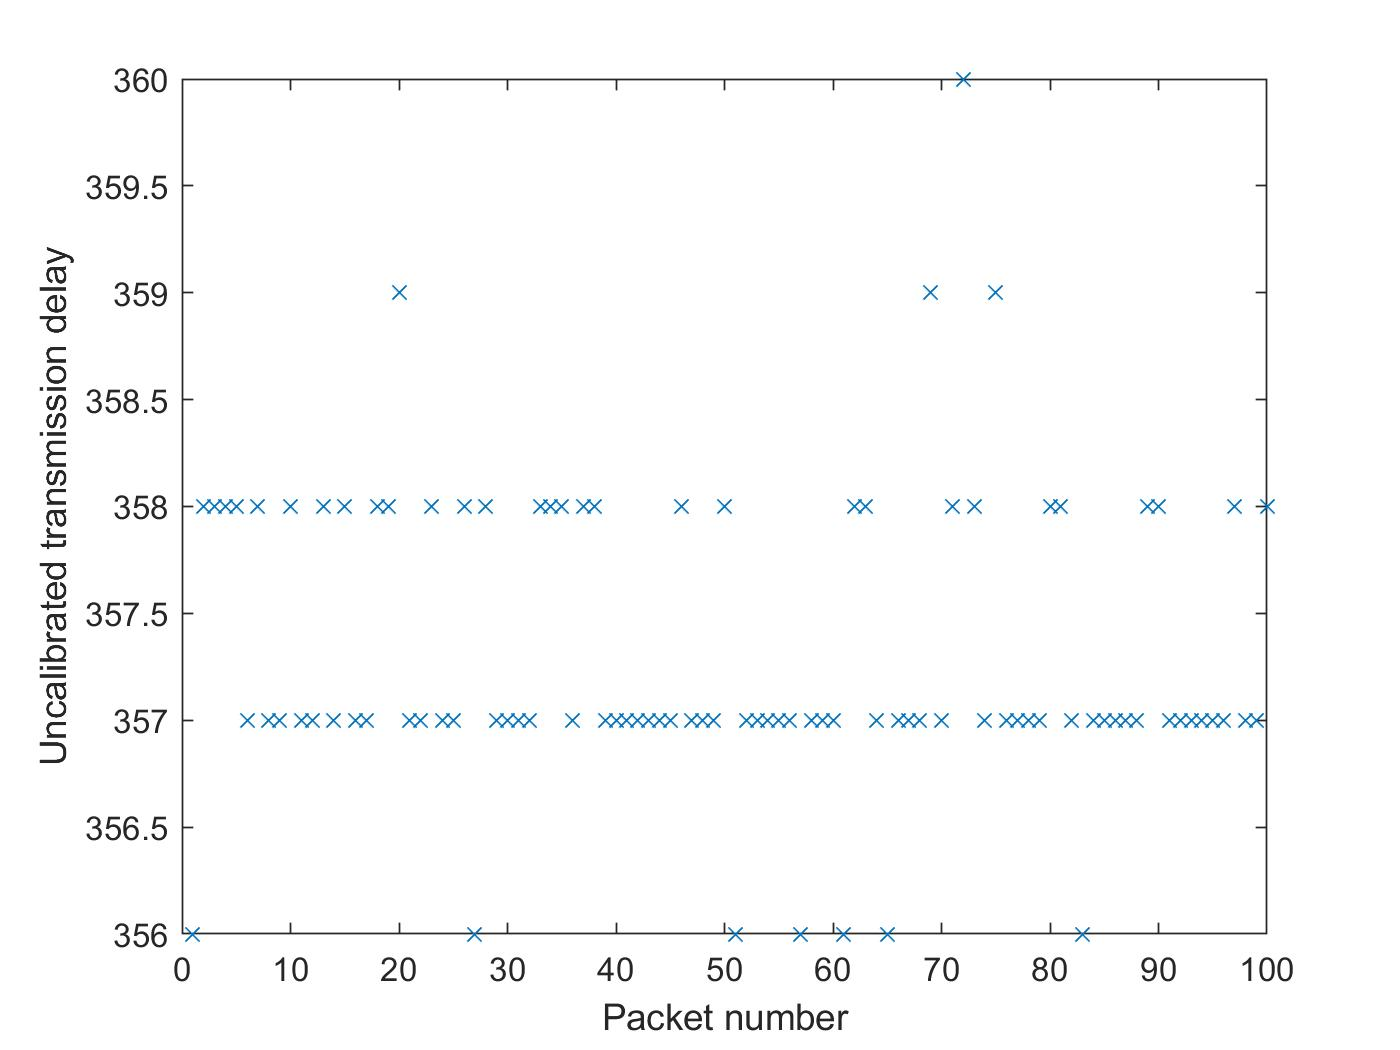
\includegraphics[width=\linewidth]{delay}
    \caption{Uncalibrated delay}
  \label{fig:td}
  \end{subfigure}
  \begin{subfigure}[t]{0.325\textwidth}
    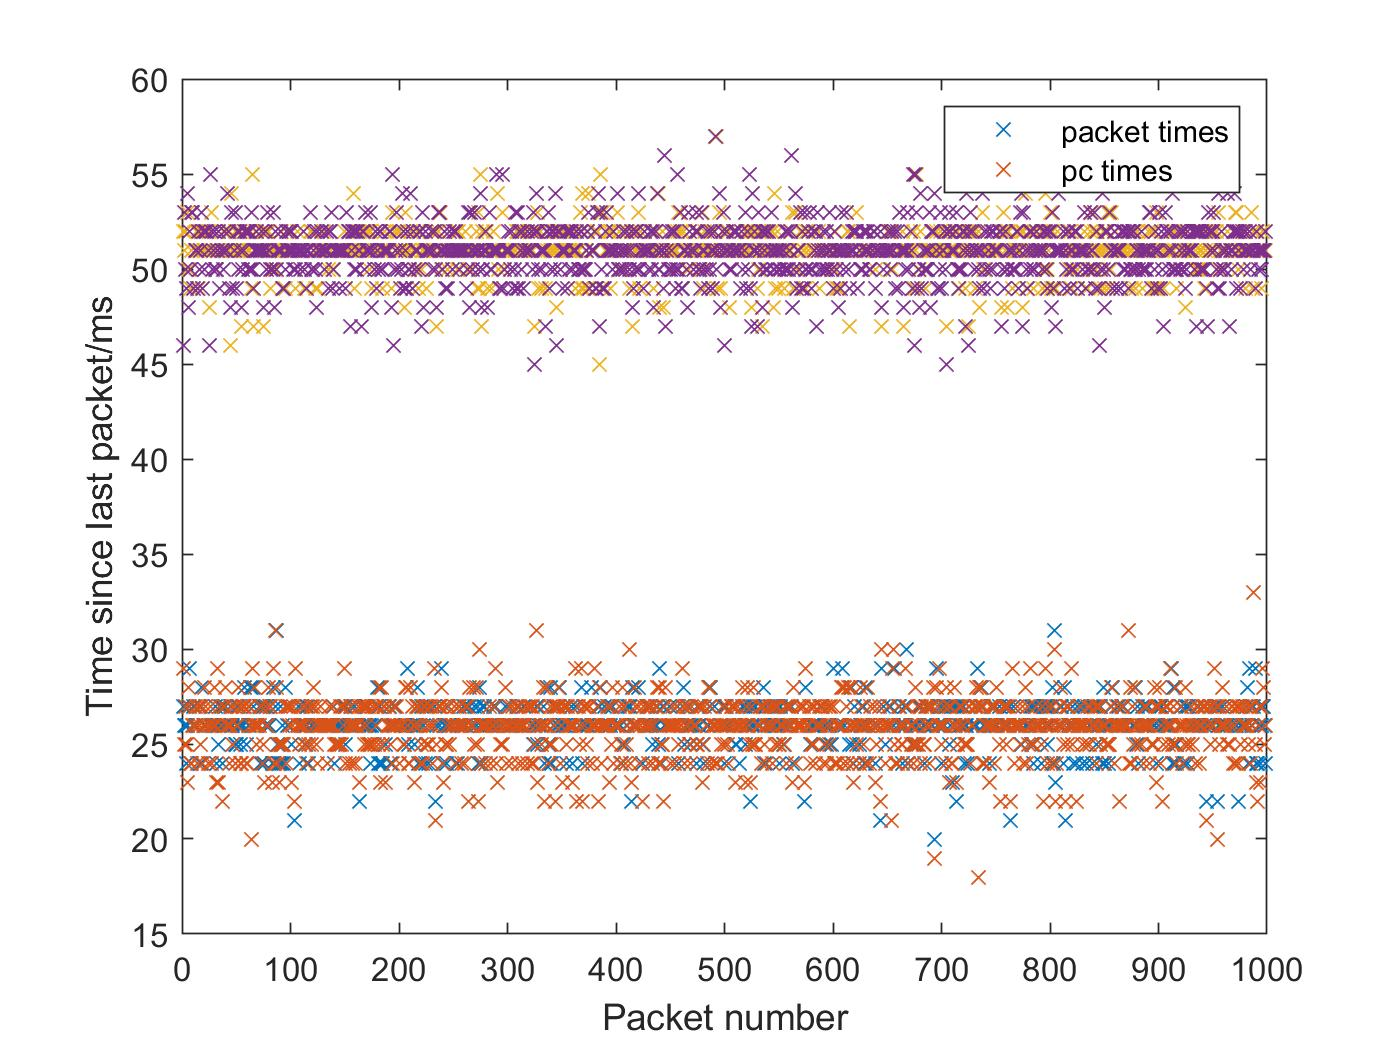
\includegraphics[width=\linewidth]{both}
    \caption{Different sampling times}
  \label{fig:ts2}
  \end{subfigure}
  \caption{Testing connecting by USB}
  \label{fig:usb}
\end{figure*}

\begin{align*}
[t, a_x, a_y ,a_z , \dot{\alpha}_x, \dot{\alpha}_y , \dot{\alpha}_z \#]
\end{align*}

UDP was chosen over serial communication protocols to take advantage of existing software and allow for wifi to easily be used again in the future if desired.

Tests were conducted to determine the reliability of this method. Figure \ref{fig:ts} shows the time between consecutive measurements on both the phone side and computer side. A mean of 50.89ms and standard deviation of 1.27ms was recorded over 1000 measurements. Variation is undesirable but this is small and times are known so won't prove problematic. A similar spread was observed at lower sampling times as shown in figure \ref{fig:ts2} where a 25ms sampling time resulted in a mean of 25.88ms and standard deviation of 1.38ms. This shows that this software is suitable if faster sampling times are required.
\newline
Due to different clocks on the computer and phone true transmission delay wasn't possible to measure. Figure \ref{fig:td} shows this uncalibrated delay. The majority of packets take one of two times to transmit with a few outliers taking $\pm$2ms. A low variation is desirable as it means actions can be applied for the correct length of time, as to not alter the trajectory away from the policy prediction.


\begin{figure}
  \centering
    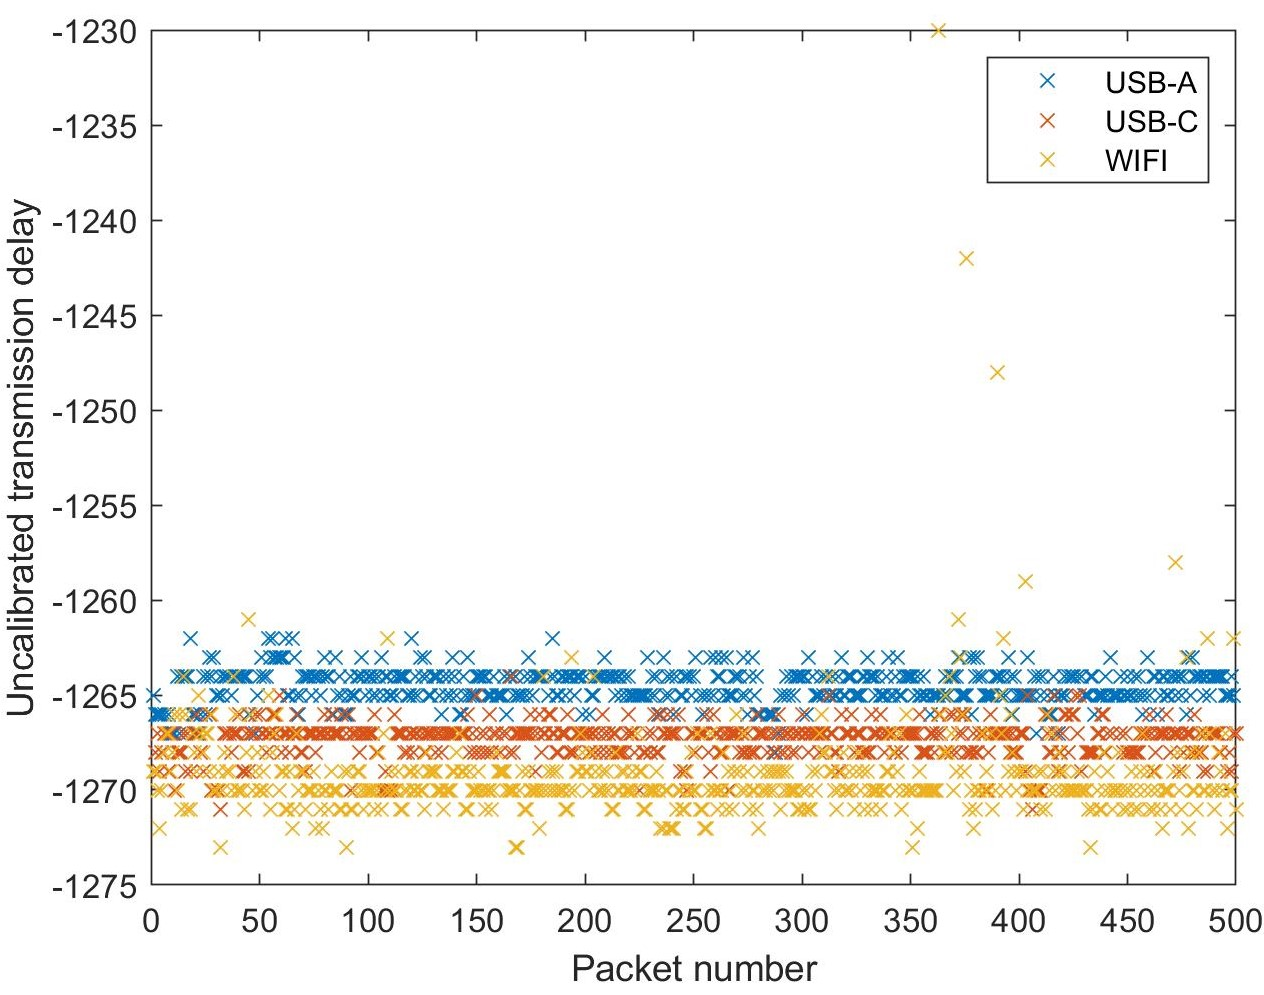
\includegraphics[width=\linewidth]{all3}
  \caption{Effect of changing transmission medium}
  \label{fig:med}
\end{figure}

\begin{table}[h]
\centering
\begin{tabular}{ c | c | c | c }
Test& USB-A & USB-C & WIFI\\ 
\midrule
1&0.99&1.05 &3.02\\
2&1.24& 1.26&1.25\\
3&1.10&1.02 &1.84\\
\end{tabular}
\caption{Transmission delay $\sigma$ in ms}
\label{table:td}
\end{table}
The delay over Three transmission mediums were compared in figure \ref{fig:med}. A smaller number on these graphs corresponds to a faster transmission. It was noticed that the difference between mediums was too large, this was explained when conducting the tests in different orders. The two clock times drifted apart after each test causing the exact delays to be incomparable, therefore flipping test order resulted in the opposite order to the figure. However, the variation in delay is what is most important when deciding method as this is what can cause unexpectedly long applied actions. Wifi showed some delays of nearly a whole time step in figure \ref{fig:med}. The standard deviation was calculated in Table \ref{table:td}. In test two the variation was almost identical amongst methods, but in the other tests wifi again showed greater variation. For this reason either USB connection is a better choice for use on the unicycle. The extra noise introduced by an extra cable effecting dynamics however may outweigh the transmission delay advantage and will need investigating. 
%------------------------------
\subsubsection{Orientation}
Imperfect starting positions in real rollouts can cause a constant offset in position throughout tests unless its determined at the start or learnt. Learning the offset is possible when training however due to the offline nature of rollouts can't be currently done on new runs. Measuring the initial orientation is therefore required, which also allows accurate uncertainty measurements ensuring predictions incorporate as much information as possible.
\begin{equation}
\begin{gathered}
\delta\textbf{a} = \textbf{a}_0 - R\hat{\textbf{a}} \\
\begin{bmatrix}
\theta \\
\psi_f \\
\end{bmatrix} = 
2 \begin{bmatrix}
tan^{-1} ( \frac{\delta\textbf{a}_x}{\sqrt{\delta\textbf{a}_y^2+\delta\textbf{a}_z^2}} )\\
-tan^{-1} ( \frac{\delta\textbf{a}_y}{\sqrt{\delta\textbf{a}_x^2+\delta\textbf{a}_z^2}} )\\
\end{bmatrix}
\label{eq:con}
\end{gathered}
\end{equation}
To calculate the initial orientation the roll and pitch angles between transformed accelerometer reading and $\textbf{a}_0 = [0,0,-1]^T$ needs to be determined. A transformation is required from the raw sensor acceleration to convert between phone and unicycle co-ordinates, this transformation being:

\begin{align*}
\textbf{a} = \begin{bmatrix}
0 & -1 & 0 \\
0 & 0 & -1\\
1 & 0 & 0 \\
\end{bmatrix}
\textbf{a}
\end{align*}



 The unicycle has only two angular DoF initially, this means that one angle can be set to 0. For this we choose yaw as this angle only depends on the starting position and is penalised when higher. The angles are measured for two seconds before initiating the rollout to estimate initial uncertainty.
\newline
Equation \ref{eq:con} calculates the initial euler orientation. This can then be easily converted to quaternion form with two quaternions rotations : (1 + 0\textbf{i}  + 0\textbf{j} + 0\textbf{k})$R_Y(\theta)R_X(\psi_f)$. Quaternions extend complex numbers to 4D and are required to accuracy keep track of repetitive rotations due to following the same mathematical rules. \cite{arsalan} Quaternion form is then used for all subsequent rotations calculated using gyroscope readings.
A rotation about axis (x,y,z) by $\alpha$ can be defined using the following unit quaternion.

\begin{gather}
\textbf{q} = cos(\frac{\alpha}{2}) + sin(\frac{\alpha}{2})(x\textbf{i} + y\textbf{j} + z\textbf{j}) \nonumber \\
\textbf{q}_{new} = \textbf{q}_{old} . \textbf{q} \nonumber
\end{gather}
  
\subsection{Raspberry Pi}
\subsubsection{Connection}

\begin{figure*}[t]
  \centering
  \begin{subfigure}[t]{0.325\textwidth}
    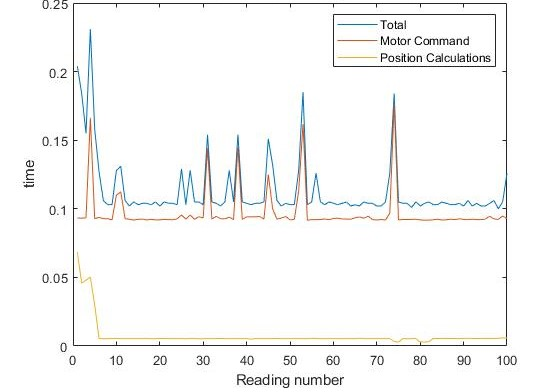
\includegraphics[width=\linewidth]{25ms_pi}
   \caption{25ms}
  \label{fig:pi25}
  \end{subfigure}
  \begin{subfigure}[t]{0.325\textwidth}
    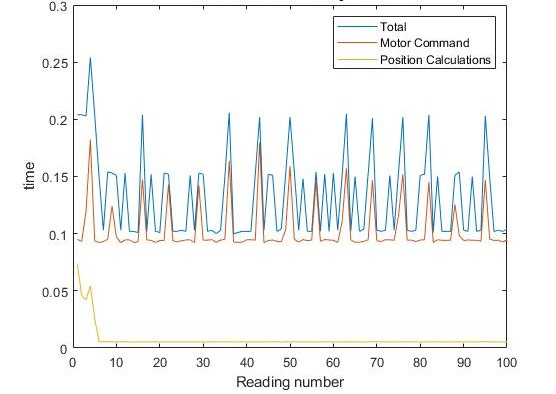
\includegraphics[width=\linewidth]{50ms_pi}
    \caption{50ms}
  \label{fig:pi50}
  \end{subfigure}
  \begin{subfigure}[t]{0.325\textwidth}
    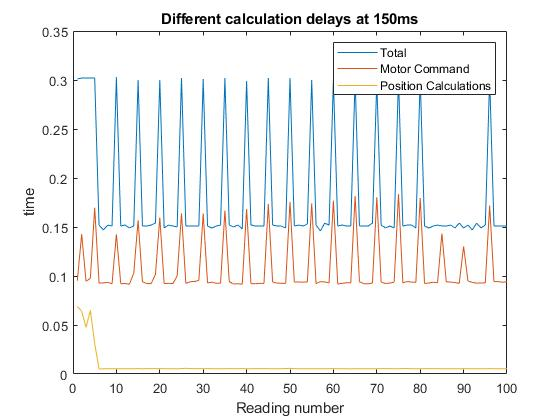
\includegraphics[width=\linewidth]{150ms_pi}
    \caption{150ms}
  \label{fig:pi150}
  \end{subfigure}
  \caption{Testing connecting from Matlab to Pi using Matlab system command}
  \label{fig:pi}
\end{figure*}
Connection to the Raspberry Pi is done using the matlab support package for Pi devices \cite{pi}. An initial set-up is required for this package. This involves connecting the Pi using a Ethernet cable, and following the package installation guide using the Raspberry Pi 3 Matlab image. Once set up the following command can be run in Matlab:

\begin{gather}
mypi = raspi('169.254.0.2', 'pi', 'raspberry') 
\end{gather}

This assigns the connection to the variable mypi, using the default IP address, username and password. This connection can then be used to send commands to the Pi:
\begin{gather}
system(mypi, 'sudo \: python \: m/filename.py')
\end{gather}
This command opens a terminal on the Rasbian OS on the Pi and runs the python file specified. Three files were used \cite{motorcmd} "enabling\_motors" , "motor\_control\_2" and "disabling\_motors". These turned on, set motor speed and turned off the motors respectively.
\newline
During testing it became apparent that there was a high degree of variation in changes to motor speed. This is unwanted because it introduces error to the dynamic model which predicts for a constant timestep. If this variation also resulted in larger timesteps then 50ms the learning ability would be drastically reduced as less data is record initially, and the dynamics are more non linear and harder to model. Figure \ref{fig:pi} shows this variation occurring when controlling the motors, for a number of different timesteps. The first few recordings took longer in each test. the execution time then settled to be at minimum 100ms, with some spikes up to 160ms. This meant that lots of sensor readings weren't being processed.
\newline
The cause of this delay was found to be the Matlab system command. This command waits for a completed message to be returned before the Matlab script proceeds. And due to the command requiring opening a new terminal, and python file each time it took at minimum 90ms. Possible solutions were tested to avoid this; adding '\&' at the end of a command stops the script waiting for a reply, however this is incompatible when executed through a Pi. The command was also ran as a batch as a sub process, this allowed the script the proceed without delay but didn't successfully control the motors. 
\newline
The implemented solution looked to minimise the need to open a new python script and terminal for each change in motor speed. For this to be implemented UDP was once again used to send motor commands. A script is ran for the duration of the rollout on the Pi, this listens to a UDP port and actions any commands sent. To initiate this command and avoid the need to wait for a response an alternative to the system command was used:

\begin{gather}
command to open a ssh window
\end{gather}

This opens a SSH connection to the Pi and a terminal on the computer. The following command is then run in this window to initiate listening on the Pi:

\begin{gather}
sudo \: python \: m/start\_rollout.py 
\end{gather}

The terminal confirms a live connection and displays motor commands sent using the following format:

\begin{gather}
[Flywheel \: Speed, \: Wheel \: Speed]
\end{gather}

The script is terminated by sending \# in this command, instead of numbers.

\begin{figure}
  \centering
    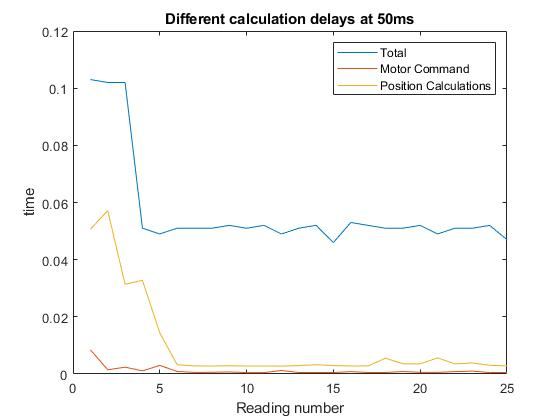
\includegraphics[width=\linewidth]{50ms_udp}
  \caption{Testing connection to Pi sending torques by UDP}
  \label{fig:piudp}
\end{figure} 

Figure \ref{fig:piudp} shows the success this method has at bringing the timestep to the desired length. Problems still occur for the initial commands which take twice as long, this was fixed by optimising the rollout loop in Matlab ensuring variables are initiated beforehand, thus decreasing the yellow line.  

%----------------------------------



\onecolumn
\subsection{Rollouts}
\begin{figure*}[t]
  \centering
  \begin{subfigure}[t]{0.325\textwidth}
    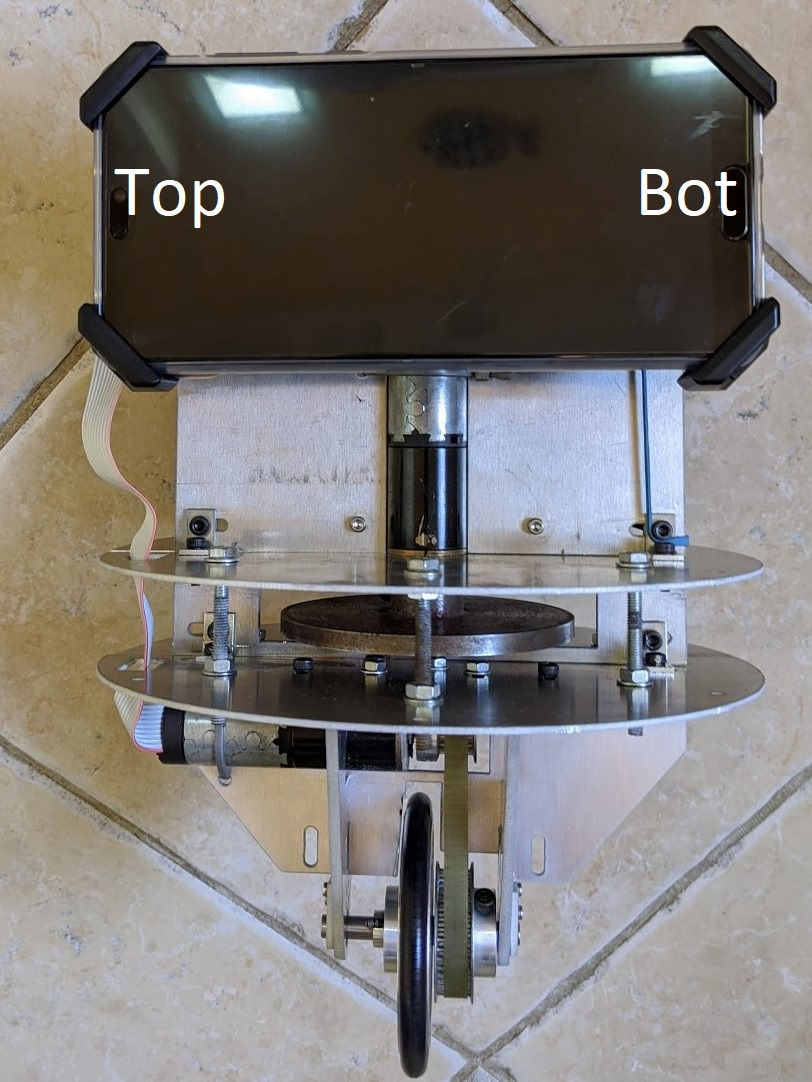
\includegraphics[height = 6.5cm]{front_lab}
   \caption{Phone set-up}
  \label{fig:set_up}
  \end{subfigure}
  \begin{subfigure}[t]{0.325\textwidth}
  \centering
    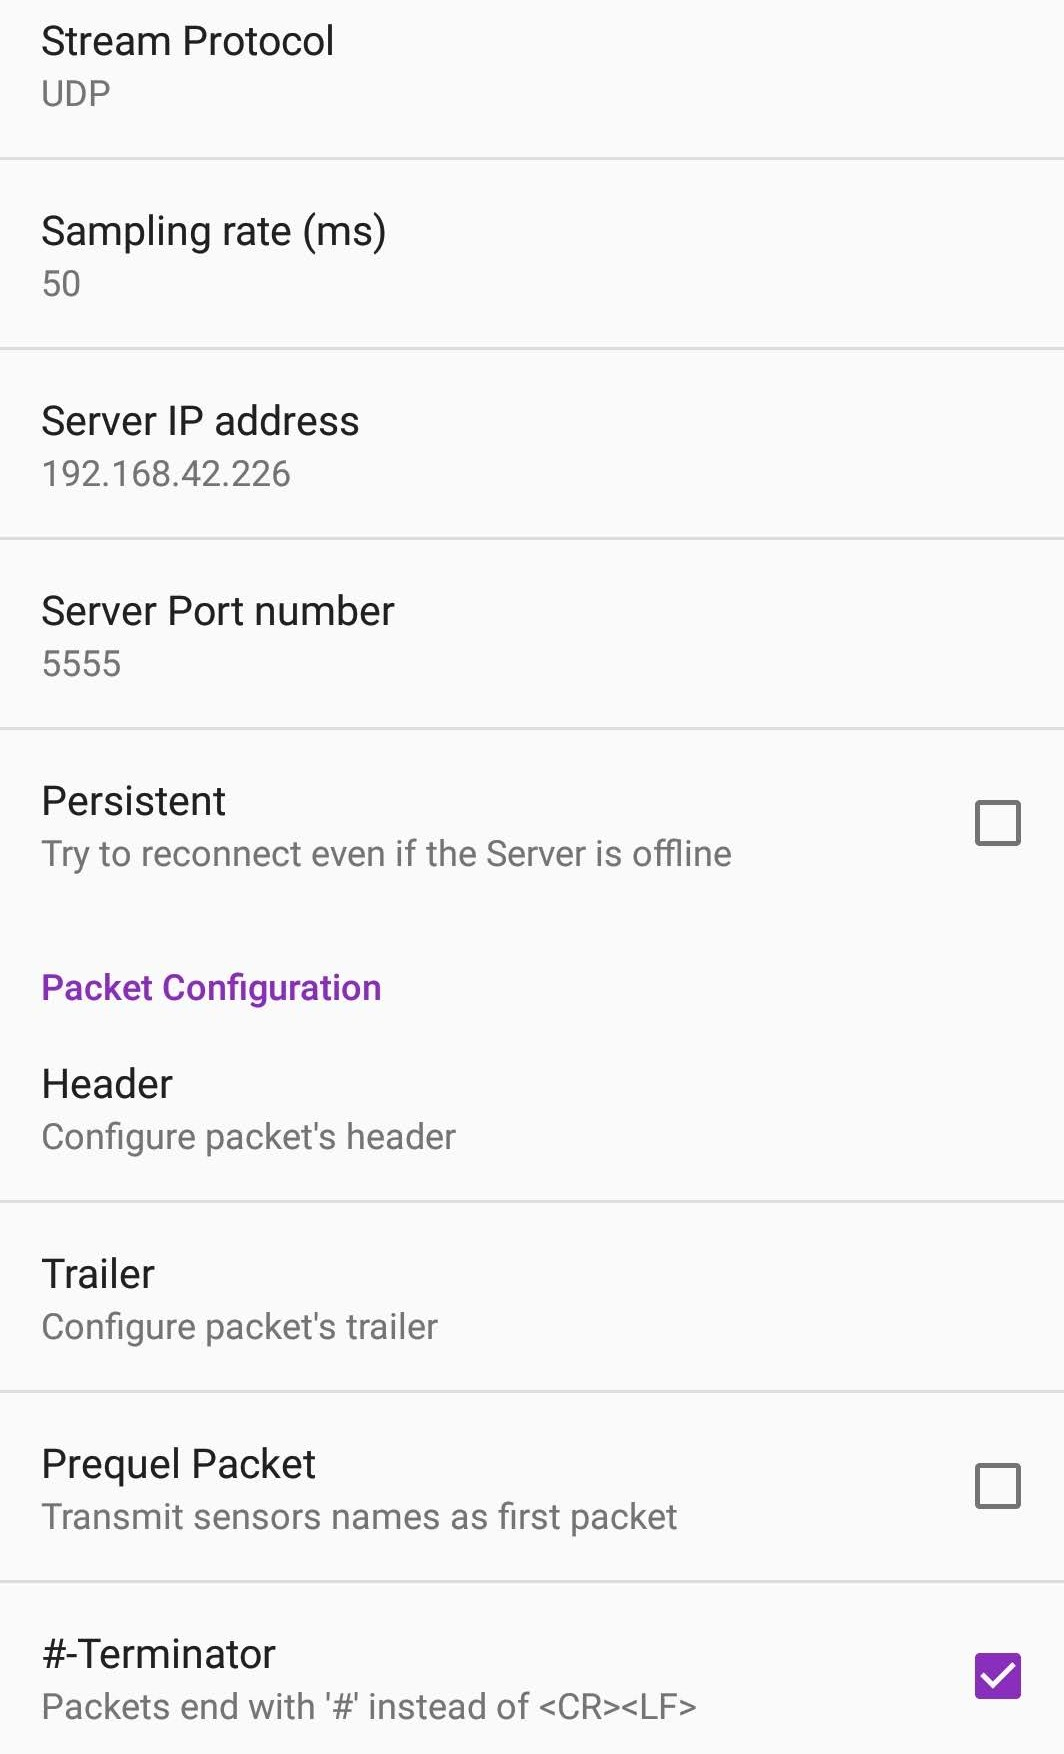
\includegraphics[height = 6.5cm]{hyperimu}
    \caption{HyperIMU settings}
  \label{fig:imuset}
  \end{subfigure}
  \begin{subfigure}[t]{0.325\textwidth}
    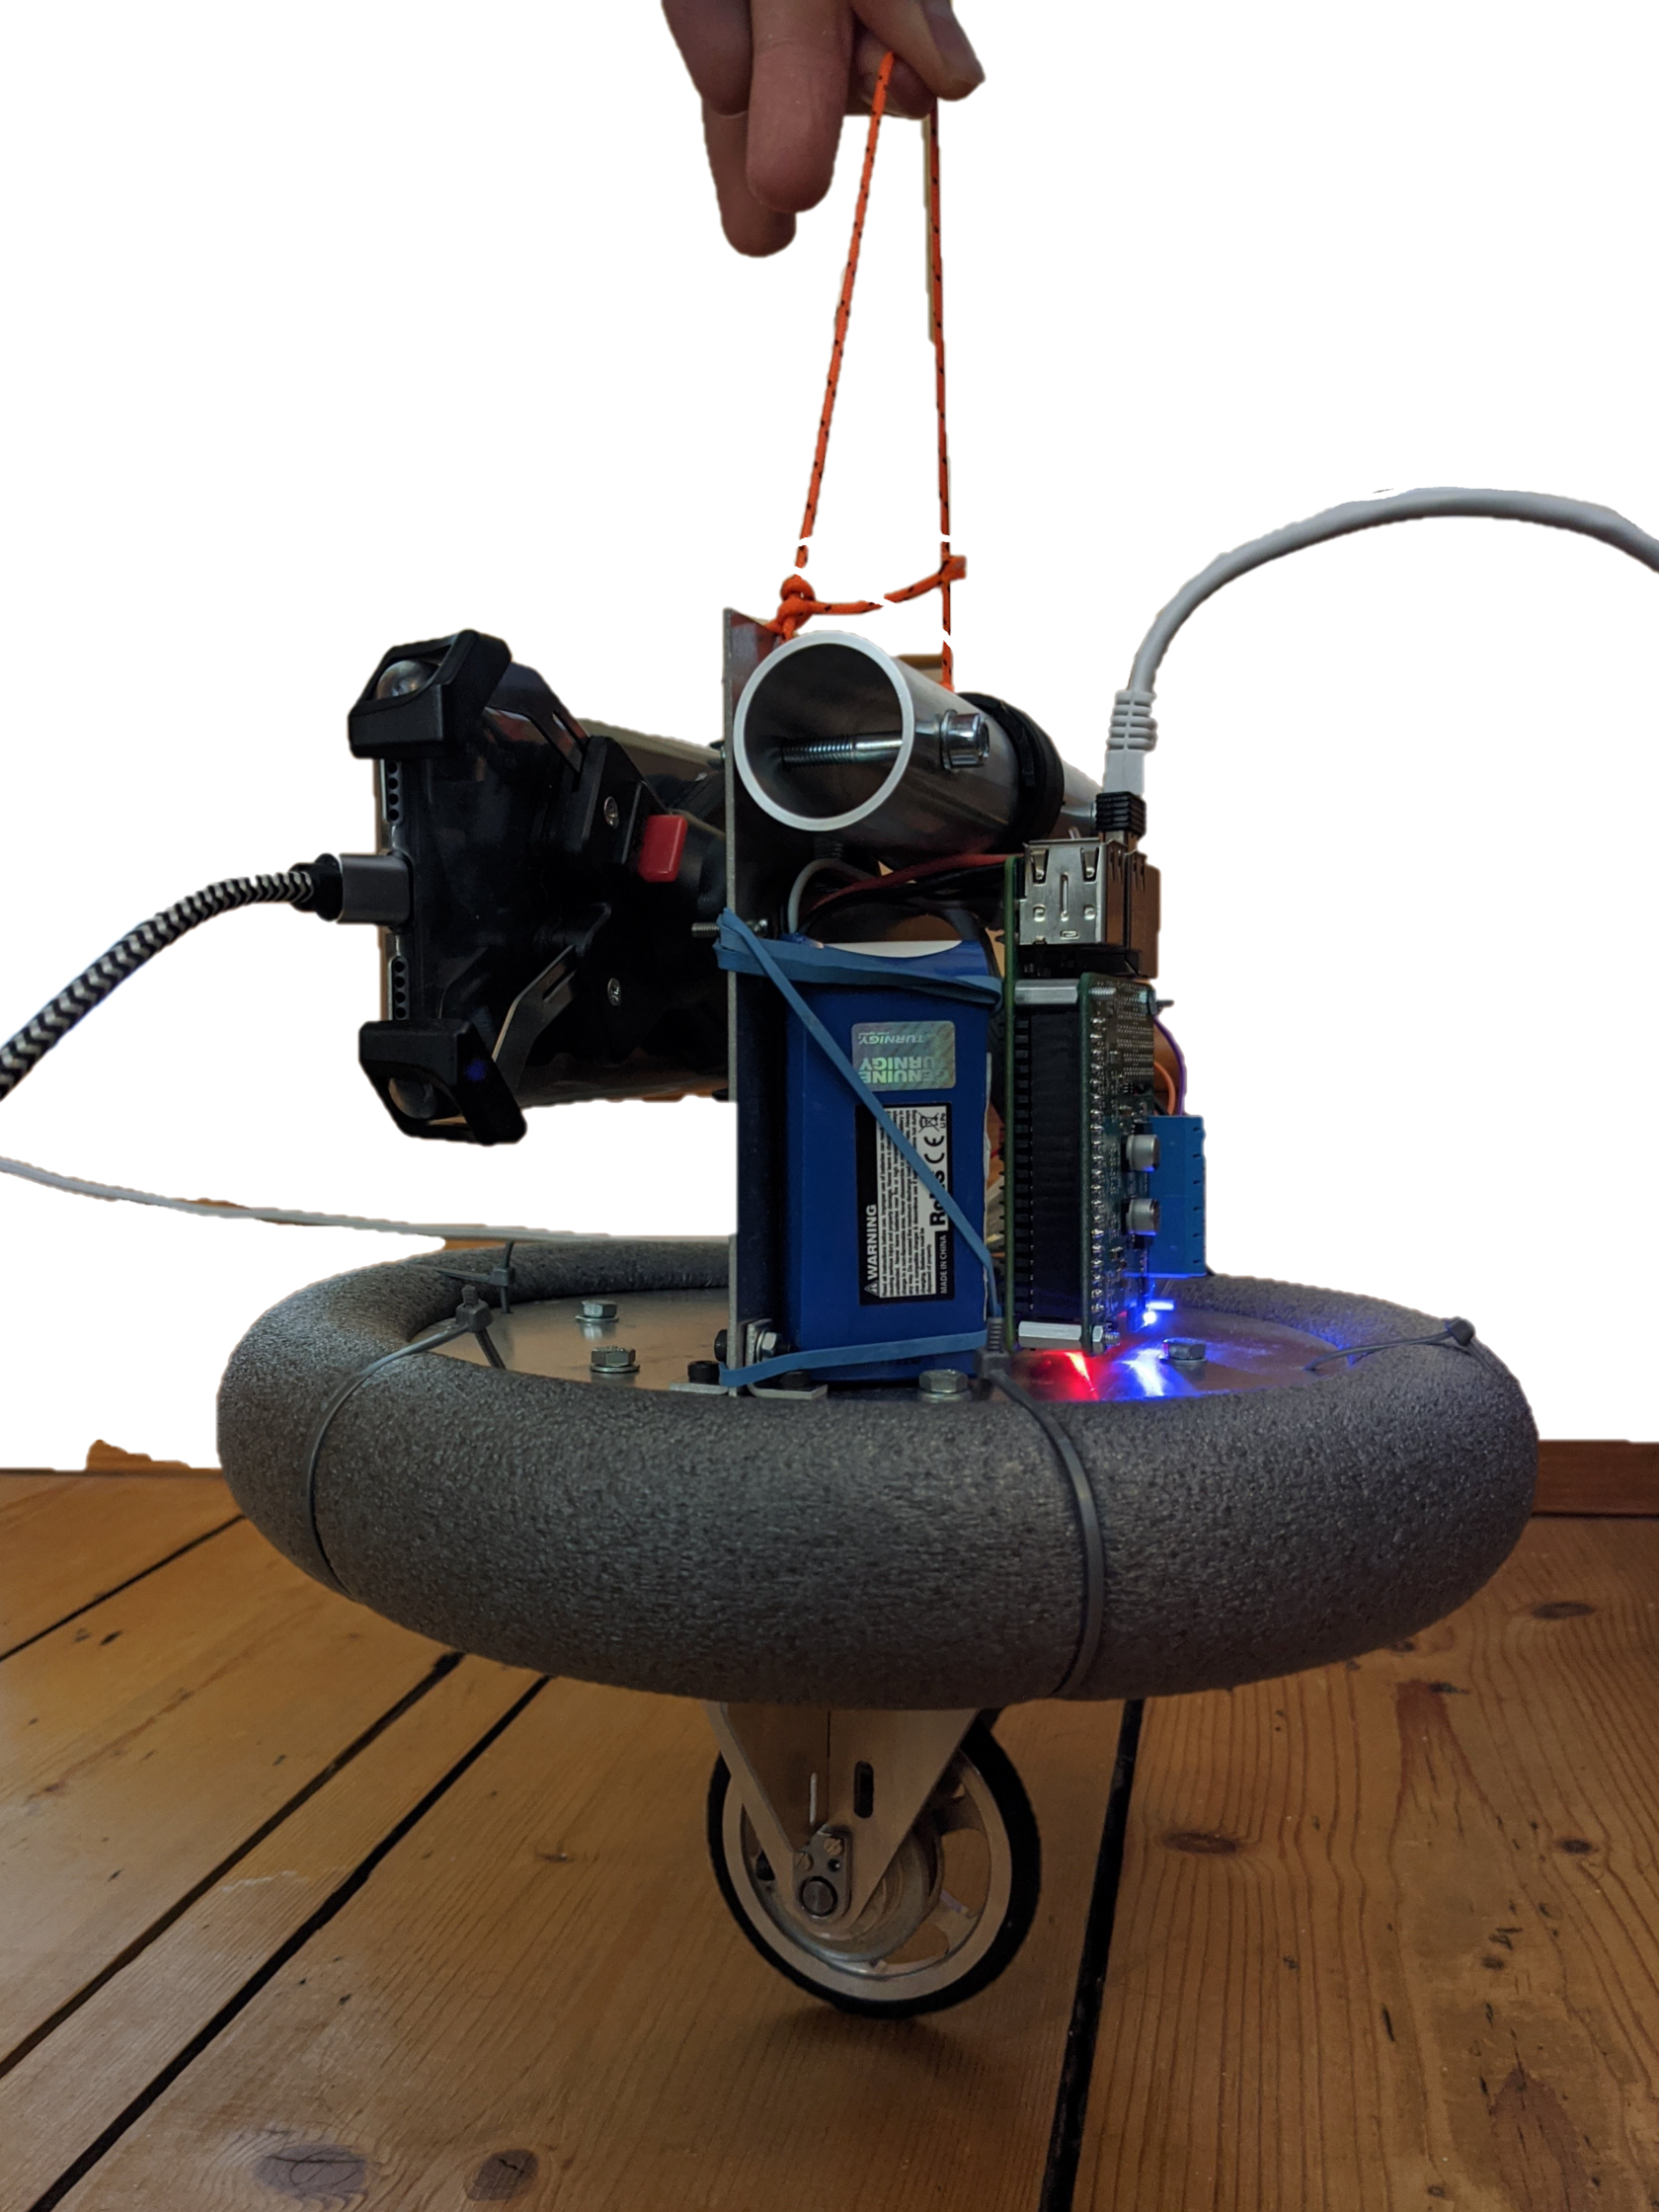
\includegraphics[height = 6.5cm]{relt}
    \caption{Release position}
  \label{fig:unirel}
  \end{subfigure}
  \caption{Steps in set-up}
  \label{fig:set_up_steps}
\end{figure*}

\subsubsection{Test Procedure}

\textbf{Mechanical Set-Up}
\begin{itemize}
\item Attach phone as in figure \ref{fig:set_up} with the top of the phone facing to the left of the unicycle. Ensure the phone attachment is vertical and secure
\item Attach the Raspberry Pi using an Ethernet cable to the computer running Matlab
\item Connect phone to computer using a USB-A/C cable
\item Connect Raspberry Pi to 5V power source, and attach on board battery
\end{itemize}

\textbf{Software Set-Up}
\begin{itemize}
\item Turn on USB tethering in the phones settings (settings/network and internet/hotspot and tethering). This often works more reliably with the phone in aeroplane mode
\item Find the ipv4 address of the attached computer. on windows this is found by typing ipconfig into a command window
\item Open HyperIMU on the phone and go to settings and enter the ipv4 address, port 5555 and desired sample rate(this is often 1ms too slow) as in figure \ref{fig:imuset}
\item Save these settings and click start logging from HyperIMU
\end{itemize}
\textbf{Rollouts}
\begin{itemize}
\item In an open flat space position the unicycle, run "doitreal.m" script from the connected computer
\item A ssh window from the computer to the Pi will then open. Typing the command "sudo python m/start\_rollout.py" will initiate listening mode on the Pi, and display all motor torques and time between subsequent messages
\item Make sure that the unicycle is being held still and vertical at this point, either by holding onto the frame or string as in figure \ref{fig:unirel}
\item The orientation is then measured for a few seconds before the motors start, at this point let go
\item After the unicycle has fallen the motors should terminate, and confirmation of a successful rollout is required in Matlab 
\item Policy optimisation and dynamics learning then ensues, the unicycle could be disconnected during this step
\item This is repeated until the desired rollouts are completed
\end{itemize}

\twocolumn
%------------------------------------------
\subsubsection{Functions}



%----------------------------
\subsubsection{Tests}

%---------------------------------
\clearpage
\begin{figure*}
  \centering
    
\includegraphics[width=\linewidth]{place}
  \caption{Optimum torque directions}
  \label{fig:quad}
\end{figure*} 
\subsection{Quadratic Controller}
All simulations and rollouts conducted so far have used a linear policy control function to determine the best action from the current state as in equation \ref{eq:lin}. There is the question of weather a linear policy is sufficient to control a unicycle. A quadratic policy of the form of equation \ref{eq:quad} may be more suitable.
\begin{equation}
\pi (\textbf{x}) = \textbf{Wx}+\textbf{p}
\label{eq:lin}
\end{equation}




Figure \ref{fig:quad} depicts the optimum action to be taken for the state space covered by [$\theta ,\psi_f$]. This ideal action is the action which minimises the distance or angle moved in that direction to return the unicycle to the desired position of [$\theta ,\psi_f$] = [0,0]. 
\newline
To correct pitch a linear policy is clearly sufficient. When the unicycle tilts forward a negative torque on the wheel is desired, and vice versa for backwards tilt. However, when looking at correcting both pitch and roll a quadratic policy appears to be required. This can be easily visualised as the flywheel rotating away from the vertical axis within each quadrant. The vertical axis corresponds to a correcting in just pitch which is linear, so a torque away from this position results in the unicycle moving towards it. This means that the direction of torque required on the flywheel alternates between each quadrant, and is effectively an XOR problem. \cite{rodrigo} 
\begin{equation}
\pi (\textbf{x}) = \textbf{x}^T\textbf{Qx} + \textbf{Wx} + \textbf{p}
\label{eq:quad}
\end{equation}
Upon further thought this may not be a problem. The optimal solution may be quadratic but by rotating the other direction the same axis where only pitch is being corrected can be achieved. This can involve a much larger angle of up to $180^{\circ}$ to work. When roll is small the two directions become more similar, and therefore shouldn't pose a problem for most states the unicycle will visit. This non optimal route allows a linear policy to work where two quadrants have the optimal torque direction and two have the sub-optimal direction. Weiser believed that with a linear controller the unicycle learnt to either always fall forward or backwards in order to remain in the optimal regions. \cite{eric}
\newline
Testing using quadratic policies could be tested in future to allow an exact evaluation of using a linear approximation. This approximation is useful because the policy parameters optimised over are greatly reduced in a linear model. Therefore training speed is far quicker.

%----------------------
\subsection{Additional Simulations}

%------------------------------------
\clearpage
\section{Conclusions}
\subsection{Progress}

%------------------------------
\subsection{Future Work}
After the further simulations has been performed and evaluated the following changes will be considered in the future:

\begin{itemize}
\item Redesign unicycle to allow for higher roll limit, different motors, greater modularity, robustness to falls and secure phone mounting.
\item Effect of independence between state variables on real rollouts.
\item Adjustments to cost function.
\end{itemize}


\subsection{Additional rollouts}


\subsection{Encoder}


\subsection{Exploration}


\subsection{Mass adjustment}


\subsection{Removing Matlab from rollouts}


%----------------------------

%------------------------------------------------------------------------
\clearpage
\begin{thebibliography}{9}
\bibitem{pilco} 
M. P. Deisenroth and C. E. Rasmussen. ''PILCO: A Model-based and Data-Efficient Approach to Policy Search''.
2011. \url{http://www.icml-2011.org/papers/323_icmlpaper.pdf.}

\bibitem{original}
Mark Mellors, Andrew Lamb and J Maciejowski. 2005 \url{roboticunicycle.info} 

\bibitem{neil}
Neil D'Souza-Mathew. ''Balancing of a Robotic Unicycle''. MEng Thesis. CUED. 2008 \url{roboticunicycle.info/documents/MyFinalReport.pdf}

\bibitem{forster}
David Forster. ''Robotic Unicycle'' MEng Thesis. CUED. 2009

\bibitem{mchut}
Andrew McHutchon, ''Machine learning for Control''. MEng Thesis. CUED. 2010

\bibitem{roderigo}
Rodrigo Queiro. ''Machine Learning for Control''. MEng Thesis. CUED. 2011
\url{https://github.com/drigz/IIB-Project/blob/master/iibproject.pdf}

\bibitem{douglass}
Alan Douglass. ''Machine Learning for Control''. MEng Thesis. CUED. 2011

\bibitem{eric}
Eric Weiser. ''Robotic Unicycle'' . MEng Thesis. CUED. 2017

\bibitem{arsalan}
Arsalan Harris. ''Robotic Unicycle'' . MEng Thesis. CUED. 2019
 
 
\bibitem{ianovir} 
Ianovir: HyperIMU app 
\url{ianovir.com/works/mobile/hyperimu/}

\bibitem{other1}
mhexrobot. 2012. \url{https://edgetriggered.wordpress.com/category/unicycle-robot/}

\bibitem{other2}
G. Daoxiong, P. Qi, Z. Guoyu, and L. Xinghui, ''Lqr control for a self-balancing unicycle
robot on inclined plane''. 2012.

\bibitem{other3}
D. W. Vos and A. H. Von Flotow, ''Dynamics and nonlinear adaptive control of an
autonomous unicycle: Theory and experiment,'' in 29th IEEE Conference on Decision
and Control, pp. 182{187, IEEE, 1990.}

\bibitem{other4}
Matthew Davis. 2019 \url{https://www.mdavis.xyz/unicycle/}

\bibitem{foam}

\bibitem{pi}

\bibitem{motorcmd}

\bibitem{mount}

\bibitem{motor}

\bibitem{gear}

\bibitem{encoder}


\end{thebibliography}



%--------------------------------------------------
\clearpage
\section{Appendix}
\subsection{Risk Assessment Review}




%------------------------------------------------

%------------------------------------------------
\end{document}
